% !TeX program = xelatex
% !TeX TXS-program:compile = txs:///xelatex/[--shell-escape]
%%%%%%%%%%%%%%%%%%%%%%%%%%%%%%%%%%%%%%%%%%%%%%%%%%%%%%%%%%%%%%%%%%%%%%%%
% Plantilla TFG/TFM
% Escuela Politécnica Superior de la Universidad de Alicante
% Realizado por: Jose Manuel Requena Plens
% Contacto: info@jmrplens.com / Telegram:@jmrplens
%%%%%%%%%%%%%%%%%%%%%%%%%%%%%%%%%%%%%%%%%%%%%%%%%%%%%%%%%%%%%%%%%%%%%%%%

% Elige si deseas optimizar la ejecución del proyecto almacenando las figuras generadas con TikZ y PGF en una carpeta (archivos/figuras-procesadas).
% 1 - Si, 2 - No
\def\OptimizaTikZ{1}

%%%%%%%%%%%%%%%%%%%%%%%%%%%%%%%%%%%%%%%%%%%%%%%%%%%%%%%%%%%%%%%%%%%%%%%%
% Plantilla TFG/TFM
% Escuela Politécnica Superior de la Universidad de Alicante
% Realizado por: Jose Manuel Requena Plens
% Contacto: info@jmrplens.com / Telegram:@jmrplens
%%%%%%%%%%%%%%%%%%%%%%%%%%%%%%%%%%%%%%%%%%%%%%%%%%%%%%%%%%%%%%%%%%%%%%%%

%%%%%%%%%%%%%%%%%%%%%%%%
% FORMATO DEL DOCUMENTO
%%%%%%%%%%%%%%%%%%%%%%%%
% scrbook es la clase de documento
% Si se desea que no haya página en blanco entre capítulos añadir "openany" en los parámetros de la clase. Sino siempre los capítulos empezarán en página impar.
\documentclass[a4paper,11pt,titlepage]{scrbook}
\KOMAoption{toc}{bib,chapterentryfill} % Opciones del índice
\usepackage{scrhack} % Previene algunos errores
% Paquete de formato para scrbook. Con marcas, linea-separador superior e inferior
\usepackage[automark,headsepline,footsepline]{scrlayer-scrpage}
\clearpairofpagestyles		% Borra los estilos por defecto
%%
% Formato y contenido de la información de cabecera y pie de página
%%
% Información de capítulo en cabecera e interno
\ihead{{\color{gray30}\scshape\small\headmark}}
% Número de página en cabecera y externo
\ohead{\normalfont\pagemark}
% Número de página en pie de página y externo. Sólo en páginas sin cabecera
\ofoot[\normalfont\pagemark]{}
%% 		
% Edición del contenido de las distintas partes de la cabecera
%%
\renewcommand{\chaptermark}[1]{\markboth{#1}{}} % Capítulo (Solo texto)
\renewcommand{\sectionmark}[1]{\markright{\thesection. #1}} % Sección (Número y texto)
\setkomafont{pagenumber}{} % Número de página (Sin nada añadido)

% Añade al índice y numera hasta la profundidad 4.
% 1:section,2:subsection,3:subsubsection,4:paragraph
\setcounter{tocdepth}{4}
\setcounter{secnumdepth}{4}
% Muestra una regla para comprobar el formato de las páginas
%\usepackage[type=upperleft,showframe,marklength=8mm]{fgruler}
% MÁRGENES DE LAS PÁGINAS
\usepackage[
  inner	=	3.0cm, % Margen interior
  outer	=	2.5cm, % Margen exterior
  top	=	2.5cm, % Margen superior
  bottom=	2.5cm, % Margen inferior
  includeheadfoot, % Incluye cabecera y pie de página en los márgenes
]{geometry}
% Valor de interlineado
\renewcommand{\baselinestretch}{1.0} % 1 línea de interlineado
% Para poder generar páginas horizontales
\usepackage{lscape}
% Ancho de la zona para comentarios en el margen. (modificado para todonotes)
\setlength{\marginparwidth}{1.9cm}

%%%%%%%%%%%%%%%%%%%%%%%%
% BIBLIOGRAFÍA
%%%%%%%%%%%%%%%%%%%%%%%%
\usepackage{apacite} % NORMA APA
\usepackage{natbib}
\usepackage{breakcites}

%%%%%%%%%%%%%%%%%%%%%%%%
% DOCUMENTO EN ESPAÑOL
%%%%%%%%%%%%%%%%%%%%%%%%
\usepackage[base]{babel}
\usepackage{polyglossia}
\setdefaultlanguage{spanish}

\addto\captionsspanish{%
  \renewcommand{\listtablename}{Índice de tablas}
  \renewcommand{\tablename}{Tabla}
  \renewcommand{\lstlistingname}{Código}
  \renewcommand{\lstlistlistingname}{Índice de \lstlistingname s}
  \renewcommand{\glossaryname}{Glosario}
  \renewcommand{\acronymname}{Acrónimos}
  \renewcommand{\bibname}{Bibliografía}%
}

%%%%%%%%%%%%%%%%%%%%%%%% 
% COLORES
%%%%%%%%%%%%%%%%%%%%%%%% 
% Biblioteca de colores
\usepackage{color}
\usepackage[dvipsnames]{xcolor}
% Otros colores definidos por el usuario
\definecolor{gray97}{gray}{.97}
\definecolor{gray75}{gray}{.75}
\definecolor{gray45}{gray}{.45}
\definecolor{gray30}{gray}{.30}
\definecolor{negro}{RGB}{0,0,0}
\definecolor{blanco}{RGB}{255,255,255}
\definecolor{dkgreen}{rgb}{0,.6,0}
\definecolor{dkblue}{rgb}{0,0,.6}
\definecolor{dkyellow}{cmyk}{0,0,.8,.3}
\definecolor{gray}{rgb}{0.5,0.5,0.5}
\definecolor{mauve}{rgb}{0.58,0,0.82}
\definecolor{deepblue}{rgb}{0,0,0.5}
\definecolor{deepred}{rgb}{0.6,0,0}
\definecolor{deepgreen}{rgb}{0,0.5,0}
\definecolor{MyDarkGreen}{rgb}{0.0,0.4,0.0}
\definecolor{bluekeywords}{rgb}{0.13,0.13,1}
\definecolor{greencomments}{rgb}{0,0.5,0}
\definecolor{redstrings}{rgb}{0.9,0,0}

%%%%%%%%%%%%%%%%%%%%%%%%
% TABLAS
%%%%%%%%%%%%%%%%%%%%%%%%
% Paquetes para tablas
\usepackage{longtable,booktabs,array,multirow,multicol,tabularx,ragged2e,array}
% Nuevos tipos de columna para tabla, se pueden utilizar como por ejemplo C{3cm} en la definición de columnas de la función tabular
\newcolumntype{L}[1]{>{\raggedright\let\newline\\\arraybackslash\hspace{0pt}}m{#1}}
\newcolumntype{C}[1]{>{\centering\let\newline\\\arraybackslash\hspace{0pt}}m{#1}}
\newcolumntype{R}[1]{>{\raggedleft\let\newline\\\arraybackslash\hspace{0pt}}m{#1}}

%%%%%%%%%%%%%%%%%%%%%%%% 
% GRAFICAS y DIAGRAMAS 
%%%%%%%%%%%%%%%%%%%%%%%% 
% Paquete para todo tipo de gráficas, diagramas, modificación de imágenes, etc
\usepackage{tikz,tikzpagenodes}
\usetikzlibrary{tikzmark,calc,shapes.geometric,arrows,backgrounds,shadings,shapes.arrows,shapes.symbols,shadows,positioning,fit,automata,patterns,intersections}
\usepackage{pgfplots}
\pgfplotsset{colormap/jet}
\pgfplotsset{compat=newest} % Compatibilidad
\usepgfplotslibrary{patchplots,groupplots,fillbetween,polar}
\usepackage{pgfplotstable}
% Guardar las figuras realizadas con Tikz y Pgf en una carpeta externa
% para agilizar el procesado y tenerlas para utilizarlas en otros
% documentos
\if\OptimizaTikZ 1
  \usepgfplotslibrary{external}
  \tikzexternalize[prefix=archivos/figuras-procesadas/] % Ruta
  \tikzset{%
    external/system call ={xelatex -enable-write18 -halt-on-error -interaction=batchmode -jobname "\image" "\texsource"},
  }
\fi

% Estilos para elementos graficos
% Cajas y cajas de texto
\tikzstyle{Caja1} = [green,very thick,rounded corners,fill=white, fill opacity=0.5]
\tikzstyle{Texto1} = [fill=white,thick,shape=circle,draw=black,inner sep=2pt,font=\sffamily,text=black]
\tikzstyle{Texto2} = [fill=white,thick,shape=rectangle,draw=black,inner sep=2pt,font=\sffamily,text=black]
\tikzstyle{Texto3} = [fill=white,thick,shape=circle,draw=black,inner sep=2pt,font=\sffamily,text=black]
% Cuadros de diagrama
\tikzstyle{rectvioleta} = [rectangle, rounded corners, text centered, draw=black, fill=blue!10]
\tikzstyle{rectnaranja} = [rectangle, minimum width=2cm, minimum height=1cm, text centered, draw=black, fill=orange!10]
\tikzstyle{romborosa} = [diamond, aspect=3, minimum width=3cm, minimum height=1cm, text centered, draw=black, fill=red!10]
\tikzstyle{rectverde} = [rectangle, minimum width=2cm, minimum height=1cm, text centered, draw=black, fill=green!10]
\tikzstyle{rectamarillo} = [rectangle, rounded corners, minimum width=2cm, minimum height=1cm, text centered, draw=black, fill=yellow!10]
% Flechas
\tikzstyle{arrow} = [thick,->,>=stealth]

%%%%%%%%%%%%%%%%%%%%%%%% 
% FIGURAS, TABLAS, ETC 
%%%%%%%%%%%%%%%%%%%%%%%% 
\usepackage{subcaption} % Para poder realizar subfiguras
\usepackage{caption} % Para aumentar las opciones de diseño
% Nombres de figuras, tablas, etc, en negrita la numeración, todo con letra small
\captionsetup{labelfont={bf,small},textfont=small}
% Paquete para modificar los espacios arriba y abajo de una figura o tabla
\usepackage{setspace}
% Define el espacio tanto arriba como abajo de las figuras, tablas
\setlength{\intextsep}{5mm}
% Para ajustar tamaños de texto de toda una tabla o grafica
% Uso: {\scalefont{0.8} \begin{...} \end{...} }
\usepackage{scalefnt}
% Redefine las tablas y figuras para eliminar el '.' entre la numeración y el texto
\renewcommand*{\figureformat}{\figurename~\thefigure}
\renewcommand*{\tableformat}{\tablename~\thetable}

%%%%%%%%%%%%%%%%%%%%%%%% 
% TEXTO
%%%%%%%%%%%%%%%%%%%%%%%%
% Paquete para poder modificar las fuente de texto
\usepackage{xltxtra}
% Cualquier tamaño de texto. Uso: {\fontsize{100pt}{120pt}\selectfont tutexto}
\usepackage{anyfontsize}
% Para modificar parametros del texto.
\usepackage{setspace}
% Paquete para posicionar bloques de texto
\usepackage{textpos}
% Paquete para realizar cajas de texto. 
% Uso: \begin{mdframed}[linecolor=red!100!black] tutexto \end{mdframed}
\usepackage{framed,mdframed}
% Para subrayar. Uso: \hlc[tucolor]{tutexto}
\newcommand{\hlc}[2][yellow]{ {\sethlcolor{#1} \hl{#2}} }

%%%%%%%%%%%%%%%%%%%%%%%% 
% OTROS
%%%%%%%%%%%%%%%%%%%%%%%%
% Para hacer una pagina horizontal. Uso: \begin{landscape} xxxx \end{lanscape}
\usepackage{lscape}
% Para incluir paginas PDF. Uso:
% \includepdf[pages={1}]{tuarchivo.pdf}
\usepackage{pdfpages}
% Para introducir url's con formato. Uso: \url{http://www.google.es}
\usepackage{url}
% Amplia muchas funciones graficas de latex
\usepackage{graphicx}
% Paquete que añade el hipervinculo en referencias dentro del documento, indice, etc
% Se define sin bordes alrededor. Uso: \ref{tulabel}
\usepackage[pdfborder={000}]{hyperref}
\usepackage{float}
\usepackage{placeins}
\usepackage{afterpage}
\usepackage{verbatim}
% Paquete para condicionales avanzados
\usepackage{xstring,xifthen}
% Paquete para realizar calculos en el código
\usepackage{calc}
% Para rotar tablas o figuras o su contenido
\usepackage{rotating}
% Para incluir comentarios en el texto. El parámetro 'disable' oculta todas las notas.
% USO: \todo{tutexto}
\usepackage[textsize=tiny,spanish,shadow,textwidth=2cm]{todonotes}
%\reversemarginpar % Descomentar si se quiere todos los comentarios en el mismo lado
% Desactiva la exportación de los ToDo y Missingfigures como figuras
\if\OptimizaTikZ 1
  \makeatletter
  \renewcommand{\todo}[2][]{\tikzexternaldisable\@todo[#1]{#2}\tikzexternalenable}
  \makeatother
  \usepackage{letltxmacro}
  \LetLtxMacro{\oldmissingfigure}{\missingfigure}
  \makeatletter
  \renewcommand{\missingfigure}[2][]{\tikzexternaldisable\oldmissingfigure[{#1}]{#2}\tikzexternalenable}
  \makeatother
\fi

%%%%%%%%%%%%%%%%%%%%%%%% 
% GLOSARIOS
%%%%%%%%%%%%%%%%%%%%%%%%
\usepackage[acronym,nonumberlist,toc]{glossaries}
\usepackage{glossary-superragged}
\newglossarystyle{modsuper}{%
  \setglossarystyle{super}%
  \renewcommand{\glsgroupskip}{}
}
\renewcommand{\glsnamefont}[1]{\textbf{#1}}


%%%%%%%%%%%%%%%%%%%%%%%% 
% COMANDOS AÑADIDOS
%%%%%%%%%%%%%%%%%%%%%%%%
% Para mostrar la fecha actual (mes año) con \Hoy
\newcommand{\MES}{%
  \ifcase\month% 0
  \or Enero% 1
  \or Febrero% 2
  \or Marzo% 3
  \or Abril% 4
  \or Mayo% 5
  \or Junio% 6
  \or Julio% 7
  \or Agosto% 8
  \or Septiembre% 9
  \or Octubre% 10
  \or Noviembre% 11
  \or Diciembre% 12
  \fi}
\newcommand{\ANYO}{\number\year}
\newcommand{\Hoy}{\MES\ \ANYO}

%%%%%%%%%%%%%%%%%%%%%%%% 
% MATEMÁTICAS
%%%%%%%%%%%%%%%%%%%%%%%%
\usepackage{mathtools,amsthm,amsfonts,amssymb,bm,mathrsfs,nicefrac,upgreek,bigints}
% Comando para añadir información de variables a las ecuaciones
% Uso: \begin{condiciones}[donde:] ....... \end{condiciones}
\newenvironment{condiciones}[1][2]
{%
#1\tabularx{\textwidth-\widthof{#1}}[t]{
>{$}l<{$} @{}>{${}}c<{{}$}@{} >{\raggedright\arraybackslash}X
}%
}
{\endtabularx\\[\belowdisplayskip]}

%%%%%
% PARÁMETROS DE FORMATO DE CODIGOS
%%%%%
% Puedes editar los formatos para ajustarlos a tu gusto
%%%%%%%%%%%%%%%%%%%%%%%%%%%%%%%%%%%%%%%%%%%%%%%%%%%%%%%%%%%%%%%%%%%%%%%%
% Plantilla TFG/TFM
% Escuela Politécnica Superior de la Universidad de Alicante
% Realizado por: Jose Manuel Requena Plens
% Contacto: info@jmrplens.com / Telegram:@jmrplens
%%%%%%%%%%%%%%%%%%%%%%%%%%%%%%%%%%%%%%%%%%%%%%%%%%%%%%%%%%%%%%%%%%%%%%%%


%%%%%%%%%%%%%%%%%%%%%%%% 
% CÓDIGO. CONFIGURACIÓN. En el siguiente bloque están los estilos.
%%%%%%%%%%%%%%%%%%%%%%%%
% Paquete para mostrar código de matlab. En caja y lineas numeradas
\usepackage[framed,numbered]{matlab-prettifier}
% Paquete mostrar código de programación de distintos lenguajes
\usepackage{listings}
\lstset{ inputencoding=utf8,
extendedchars=true,
frame=single, % Caja donde se ubica el código
backgroundcolor=\color{gray97}, % Color del fondo de la caja
rulesepcolor=\color{black},
boxpos=c,
abovecaptionskip=-4pt,
aboveskip=12pt,
belowskip=0pt,
lineskip=0pt,
framerule=0pt,
framextopmargin=4pt,
framexbottommargin=4pt,
framexleftmargin=11pt,
framexrightmargin=0pt,
linewidth=\linewidth,
xleftmargin=\parindent,
framesep=0pt,
rulesep=.4pt,
stringstyle=\ttfamily,
showstringspaces = false,
showspaces = false,
showtabs = false,
columns=fullflexible,
basicstyle=\small\ttfamily,
commentstyle=\color{gray45},
keywordstyle=\bfseries,
tabsize=4,
numbers=left,
numbersep=1pt,
numberstyle=\tiny\ttfamily\color{gray75},
numberfirstline = false,
breaklines=true,
postbreak=\mbox{\textcolor{red}{$\hookrightarrow$}\space}, % Flecha al saltar de linea
prebreak=\mbox{\textcolor{red}{$\hookleftarrow$}\space}, % Flecha al saltar de linea
literate=
  {á}{{\'a}}1 {é}{{\'e}}1 {í}{{\'i}}1 {ó}{{\'o}}1 {ú}{{\'u}}1
  {Á}{{\'A}}1 {É}{{\'E}}1 {Í}{{\'I}}1 {Ó}{{\'O}}1 {Ú}{{\'U}}1
  {à}{{\`a}}1 {è}{{\`e}}1 {ì}{{\`i}}1 {ò}{{\`o}}1 {ù}{{\`u}}1
  {À}{{\`A}}1 {È}{{\'E}}1 {Ì}{{\`I}}1 {Ò}{{\`O}}1 {Ù}{{\`U}}1
  {ä}{{\"a}}1 {ë}{{\"e}}1 {ï}{{\"i}}1 {ö}{{\"o}}1 {ü}{{\"u}}1
  {Ä}{{\"A}}1 {Ë}{{\"E}}1 {Ï}{{\"I}}1 {Ö}{{\"O}}1 {Ü}{{\"U}}1
  {â}{{\^a}}1 {ê}{{\^e}}1 {î}{{\^i}}1 {ô}{{\^o}}1 {û}{{\^u}}1
  {Â}{{\^A}}1 {Ê}{{\^E}}1 {Î}{{\^I}}1 {Ô}{{\^O}}1 {Û}{{\^U}}1
  {œ}{{\oe}}1 {Œ}{{\OE}}1 {æ}{{\ae}}1 {Æ}{{\AE}}1 {ß}{{\ss}}1
  {ű}{{\H{u}}}1 {Ű}{{\H{U}}}1 {ő}{{\H{o}}}1 {Ő}{{\H{O}}}1
  {ç}{{\c c}}1 {Ç}{{\c C}}1 {ø}{{\o}}1 {å}{{\r a}}1 {Å}{{\r A}}1
  {€}{{\euro}}1 {£}{{\pounds}}1 {«}{{\guillemotleft}}1
  {»}{{\guillemotright}}1 {ñ}{{\~n}}1 {Ñ}{{\~N}}1 {¿}{{?`}}1,
  }

% Intenta no dividir los códigos en diferentes paginas si es posible
\lstnewenvironment{listing}[1][]
   {\lstset{#1}\pagebreak[0]}{\pagebreak[0]}

% Formato de títulos de los códigos
\DeclareCaptionFont{white}{\color{white}}
\DeclareCaptionFormat{listing}{\colorbox{gray}{\parbox{\textwidth - 2\fboxsep}{#1#2#3}}}
\captionsetup[lstlisting]{format=listing,labelfont=white,textfont=white,font= scriptsize}


%%%%%%%%%%%%%%%%%%%%%%%% 
% CÓDIGO. ESTILOS. Ajústalos a tu gusto
%%%%%%%%%%%%%%%%%%%%%%%%
\lstdefinestyle{Consola}
	{
	basicstyle=\scriptsize\bfseries\ttfamily,
	}
   
\lstdefinestyle{C}
	{
	basicstyle=\scriptsize,
	language=C,
	}
\lstdefinestyle{C-color}
	{
  	breaklines=true,
  	language=C,
  	basicstyle=\scriptsize,
  	keywordstyle=\bfseries\color{green!40!black},
  	commentstyle=\itshape\color{purple!40!black},
  	identifierstyle=\color{blue},
  	stringstyle=\color{orange},
    }
\lstdefinestyle{CSharp}
	{
	basicstyle=\scriptsize,
	language=[Sharp]C,
	escapeinside={(*@}{@*)},
	keywordstyle=\bfseries,
	}
\lstdefinestyle{CSharp-color}
	{
	basicstyle=\scriptsize,
	language=[Sharp]C,
	escapeinside={(*@}{@*)},
	commentstyle=\color{greencomments},
	keywordstyle=\color{bluekeywords}\bfseries,
	stringstyle=\color{redstrings},
	}
\lstdefinestyle{C++}
	{
	basicstyle=\scriptsize,
	language=C++,
 	}
 	
\lstdefinestyle{C++-color}
	{
  	breaklines=true,
  	language=C++,
  	basicstyle=\scriptsize,
  	keywordstyle=\bfseries\color{green!40!black},
  	commentstyle=\itshape\color{purple!40!black},
  	identifierstyle=\color{blue},
  	stringstyle=\color{orange},
    }
    
\lstdefinestyle{PHP}
	{
	basicstyle=\scriptsize,
	language=PHP,
	}
	
\lstdefinestyle{PHP-color}
	{
	basicstyle=\scriptsize,
	language=PHP,
	keywordstyle    = \color{dkblue},
  	stringstyle     = \color{red},
  	identifierstyle = \color{dkgreen},
  	commentstyle    = \color{gray},
  	emph            =[1]{php},
  	emphstyle       =[1]\color{black},
  	emph            =[2]{if,and,or,else},
  	emphstyle       =[2]\color{dkyellow}
  }
  
\lstdefinestyle{Matlab}
	{
	basicstyle=\scriptsize,
	language=Matlab,
	numberstyle=\tiny\ttfamily\color{gray75},
	}
	
\lstdefinestyle{Matlab-color}
	{
	style = Matlab-editor,
	basicstyle=\scriptsize,
	numberstyle=\tiny\ttfamily\color{gray75},
	}
	
\lstdefinestyle{Latex}
	{
	language=[LaTeX]{Tex},
    basicstyle=\scriptsize,
    literate={\$}{{{\bfseries\$}}}1,
    alsoletter={\\,*,\&},
    emph =[1]{\\begin,\\end,\\caption,\\label,\\centering,\\FloatBarrier,
              \\lstinputlisting,\\scalefont,\\addplot,\\input,
              \\legend,\\item,\\subitem,\\includegraphics,\\textwidth,
              \\section,\\subsection,\\subsubsection,\\paragraph,
              \\cite,\\citet,\\citep,\\gls,\\bibliographystyle,\\url,
              \\citet*,\\citep*,\\todo,\\missingfigure,\\footnote},
  	emphstyle =[1]\bfseries,
  	emph = [2]{equation,subequations,eqnarray,figure,subfigure,
  			   condiciones,flalign,tikzpicture,axis,lstlisting,
  			   itemize,description
  			   },
  	emphstyle =[2]\bfseries,
    numbers=none,
	}
	
\lstdefinestyle{Latex-color}
	{
	language=[LaTeX]{Tex},
    basicstyle=\scriptsize,
    commentstyle=\color{dkgreen},
    identifierstyle=\color{black},
    literate={\$}{{{\bfseries\color{Dandelion}\$}}}1, % Colorea el simbolo dollar
    alsoletter={\\,*,\&},
    emph =[1]{\\begin,\\end,\\caption,\\label,\\centering,\\FloatBarrier,
              \\lstinputlisting,\\scalefont,\\addplot,\\input,
              \\legend,\\item,\\subitem,\\includegraphics,\\textwidth,
              \\section,\\subsection,\\subsubsection,\\paragraph,
              \\cite,\\citet,\\citep,\\gls,\\bibliographystyle,\\url,
              \\citet*,\\citep*,\\todo,\\missingfigure,\\footnote},
  	emphstyle =[1]\bfseries\color{RoyalBlue},
  	emph = [2]{equation,subequations,eqnarray,figure,subfigure,
  			   condiciones,flalign,tikzpicture,axis,lstlisting,
  			   itemize,description
  			   },
  	emphstyle =[2]\bfseries,
    numbers=none,
	}
\lstdefinestyle{Java}
{
	basicstyle=\scriptsize,
	language=Java,
}

\lstdefinestyle{Java-color}
{
	basicstyle=\scriptsize,
	language=Java,
  	keywordstyle=\color{blue},
  	commentstyle=\color{dkgreen},
  	stringstyle=\color{mauve},
}
\lstdefinestyle{Python}
{
	language=Python,
	basicstyle=\scriptsize,
	otherkeywords={self},  
	keywordstyle=\bfseries,     
	emphstyle=\bfseries,    
	emph={MyClass,__init__},         
}

\lstdefinestyle{Python-color}
{
	language=Python,
	basicstyle=\scriptsize,
	otherkeywords={self},          
	keywordstyle=\bfseries\color{deepblue},
	emph={MyClass,__init__},         
	emphstyle=\bfseries\color{deepred},    
	stringstyle=\color{deepgreen},
}
\lstdefinestyle{R}
{
	language=R,                     
  	basicstyle=\scriptsize,
  	keywordstyle=\bfseries, 
}
\lstdefinestyle{R-color}
{
	language=R,                     
  	basicstyle=\scriptsize,
  	keywordstyle=\bfseries\color{RoyalBlue}, 
  	commentstyle=\color{YellowGreen},
  	stringstyle=\color{ForestGreen}  
}


%%%%%
% DEFINICION DE CONCEPTOS
%%%%
% Uso ejemplo: \begin{ejemplo} tucontenido \end{ejemplo} 
\newtheorem{teorema}{Teorema}[chapter]
\newtheorem{ejemplo}{Ejemplo}[chapter]
\newtheorem{definicion}{Definición}[chapter]



\newcommand{\titulo}{Prognosticating Physique: Machine Learning for Future Body Shape Estimations in Weight Loss}

% Sugerencias de ChatGPT:
% "Anticipating Body Shape Transformations: A Neural Network Approach to Weight Loss Predictions"
% "Prognosticating Physique: Machine Learning for Future Body Shape Estimations in Weight Loss"
% "A Time Series Approach to Body Shape Prediction in Weight Loss Scenarios"
% "From Present to Future Physique: Predicting Body Shape Changes Through Weight Loss"
% "Generative Models for Future Human Body Shape Estimation During Weight Loss"
% "Exploring the Future Self: AI-powered Predictions of Body Shape Changes in Weight Loss"
% "Machine Learning Meets Fitness: A Study on Predicting Body Shape Post Weight Loss"
% "Neural Networks in Nutritional Science: Predicting Future Body Shapes in Weight Loss"
% "Predictive Modeling of Human Body Transformation in Weight Loss Journey"
% "The Future of Fitness: A Neural Network-Based Prediction of Post-Weight-Loss Body Shapes"

\newcommand{\subtitulo}{Utilizing AI to Anticipate Physical Changes in Weight Loss Regimens}

% Sugerencias de ChatGPT:
% "Harnessing the Power of Machine Learning to Visualize Health Transformations"
% "A Deep Dive into Time Series Prediction of Human Physique"
% "Utilizing AI to Anticipate Physical Changes in Weight Loss Regimens"
% "An Innovative Approach to Forecasting Body Shape Transformations"
% "A Novel Methodology for Visualizing Personalized Weight Loss Outcomes"
% "Exploring the Potential of Neural Networks in Personalized Fitness"
% "Advancing Health Predictions with Generative Neural Networks"
% "Bridging Machine Learning and Fitness: Towards a Personalized Future"
% "Embracing AI for Personalized Predictions in Weight Loss Journeys"
% "Exploring the Intersection of AI and Health: Next-Level Personal Fitness Predictions"

\newcommand{\miNombre}{Pablo Ramón Guevara}
\newcommand{\miEmail}{prg54@alu.ua.es}

\newcommand{\miTutor}{Jorge Azorín López}
\newcommand{\miTutorB}{Andrés Fuster Guilló}
\newcommand{\departamentoTutor}{Department of Computer Science and Technology}
\newcommand{\departamentoTutorB}{Department of Computer Science and Technology}

\newcommand{\miFacultad}{Escuela Politécnica Superior}
\newcommand{\miFacultadCorto}{EPS UA}
\newcommand{\miUniversidad}{\protect{Universidad de Alicante}}
\newcommand{\miUbicacion}{Alicante}

\def\IDtitulo{4}

%%%%%%%%%%%%%%%%%%%%%%%%%%%%%%%%%%%%%%%%%%%%%%%%%%%%%%%%%%%%%%%%%%%%%%%%
% Plantilla TFG/TFM
% Escuela Politécnica Superior de la Universidad de Alicante
% Realizado por: Jose Manuel Requena Plens
% Contacto: info@jmrplens.com / Telegram:@jmrplens
%%%%%%%%%%%%%%%%%%%%%%%%%%%%%%%%%%%%%%%%%%%%%%%%%%%%%%%%%%%%%%%%%%%%%%%%

%%%%%%%%%%%%%%%%%%%%%%%% 
% COLORES DE GRADOS.
% Si el color de la titulación ha cambiado, modifícalo en las lineas siguientes.
%%%%%%%%%%%%%%%%%%%%%%%%
% Grados
\definecolor{teleco}{RGB}{32,2,116}			% Teleco
\definecolor{civil}{RGB}{201,56,140}			% Civil
\definecolor{quimica}{RGB}{41,199,255}		% Química
\definecolor{informatica}{RGB}{0,128,255}	% Informatica
\definecolor{multimedia}{RGB}{239,206,53}	% Multimedia
\definecolor{arquitecnica}{RGB}{0,179,148}	% Arquitectura técnica
\definecolor{arquitectura}{RGB}{181,0,0}		% Arquitectura
\definecolor{robotica}{RGB}{255,255,128}		% Robótica
% Másteres
\definecolor{masterteleco}{RGB}{32,2,116}	% Teleco
\definecolor{caminos}{RGB}{201,56,140}		% Caminos, Canales y Puertos
\definecolor{gestedif}{RGB}{50,120,50}		% Gestión Edificación
\definecolor{desweb}{RGB}{250,43,22}			% Desarrollo Web
\definecolor{mataguaterre}{RGB}{210,250,50}	% Materiales, Agua, Terreno
\definecolor{masterinfor}{RGB}{0,128,255}	% Informática
\definecolor{autorobo}{RGB}{83,145,201}		% Automática y Robótica
\definecolor{prevencion}{RGB}{0,100,0}		% Prevención Riesgos
\definecolor{gestionagua}{RGB}{7,138,197}	% Gestión Agua
\definecolor{moviles}{RGB}{121,11,21}		% Aplicaciones Móviles
\definecolor{masterquimica}{RGB}{41,199,255}	% Quimica
\definecolor{ciberseguridad}{RGB}{9,111,192}	% Ciberseguridad
\definecolor{geologica}{RGB}{245,125,0}		% Ingeniería Geológica

% Logotipos comunes de todas las titulaciones
\newcommand{\logoFacultad}{include/logos-universidad/LogoEPSNegro}
\newcommand{\logoUniversidad}{include/logos-universidad/LogoUANegro}
\newcommand{\logoUniversidadPortada}{include/logos-universidad/LogoUABlanco}

% Colores generales
\definecolor{negro}{RGB}{0,0,0}
\definecolor{blanco}{RGB}{255,255,255}
%%%%%%%%%%%%%%%%%%%%%%%% 
% CONDICIONALES. SEGUN LA ID ELEGIDA EN EL .TEX PRINCIPAL
% Según el ID seleccionado en TFG_EPS_UA.tex se configurará el nombre de la titulación, logotipos y color.
% Si tu titulación no esta correctamente definida cambia las imágenes que se definen para tu titulación en las lineas de abajo
% Si deseas añadir mas titulaciones ve al final de este archivo
%%%%%%%%%%%%%%%%%%%%%%%%
% Grados
	\if\IDtitulo 1 % Teleco
		% Logos
		\newcommand{\logoFacultadPortada}{include/logos-universidad/LogoEPSBlanco}
		\newcommand{\logoGradoPortada}{include/logos-titulaciones/LogoTelecoBlanco}
		\newcommand{\logoGrado}{include/logos-titulaciones/LogoTelecoNegro}
		% Texto
		\newcommand{\miGrado}{Grado en Ingeniería en Sonido e Imagen en Telecomunicación}
		\newcommand{\tipotrabajo}{Trabajo Fin de Grado}
		% Color
		\newcommand{\colorgrado}{teleco}
		\newcommand{\colortexto}{blanco}
	\else \if\IDtitulo 2 % Civil
		\newcommand{\logoFacultadPortada}{include/logos-universidad/LogoEPSBlanco}
		\newcommand{\logoGradoPortada}{include/logos-titulaciones/LogoCivilBlanco}
		\newcommand{\logoGrado}{include/logos-titulaciones/LogoCivilNegro}
		% Texto
		\newcommand{\miGrado}{Grado en Ingeniería Civil}
		\newcommand{\tipotrabajo}{Trabajo Fin de Grado}
		% Color
		\newcommand{\colorgrado}{civil}
		\newcommand{\colortexto}{blanco}
	\else \if\IDtitulo 3 % Quimica
		% Logos
		\newcommand{\logoFacultadPortada}{include/logos-universidad/LogoEPSNegro}
		\newcommand{\logoGradoPortada}{include/logos-titulaciones/LogoQuimicaNegro}
		\newcommand{\logoGrado}{include/logos-titulaciones/LogoQuimicaNegro}
		% Texto
		\newcommand{\miGrado}{Grado en Ingeniería Química}
		\newcommand{\tipotrabajo}{Trabajo Fin de Grado}
		% Color
		\newcommand{\colorgrado}{quimica}
		\newcommand{\colortexto}{negro}
	\else \if\IDtitulo 4 % Informatica
		% Logos
		\newcommand{\logoFacultadPortada}{include/logos-universidad/LogoEPSBlanco}
		\newcommand{\logoGradoPortada}{include/logos-titulaciones/LogoInformaticaBlanco}
		\newcommand{\logoGrado}{include/logos-titulaciones/LogoInformaticaNegro}
		% Texto
		\newcommand{\miGrado}{Grado en Ingeniería Informática}
		\newcommand{\tipotrabajo}{Trabajo Fin de Grado}
		% Color
		\newcommand{\colorgrado}{informatica}
		\newcommand{\colortexto}{blanco}
	\else \if\IDtitulo 5 % Multimedia
		% Logos
		\newcommand{\logoFacultadPortada}{include/logos-universidad/LogoEPSNegro}
		\newcommand{\logoGradoPortada}{include/logos-titulaciones/LogoMultimediaNegro}
		\newcommand{\logoGrado}{include/logos-titulaciones/LogoMultimediaNegro}
		% Texto
		\newcommand{\miGrado}{Grado en Ingeniería Multimedia}
		\newcommand{\tipotrabajo}{Trabajo Fin de Grado}
		% Color
		\newcommand{\colorgrado}{multimedia}
		\newcommand{\colortexto}{negro}
	\else \if\IDtitulo 6 % Arquitectura Tecnica
		% Logos
		\newcommand{\logoFacultadPortada}{include/logos-universidad/LogoEPSBlanco}
		\newcommand{\logoGradoPortada}{include/logos-titulaciones/LogoArqTecnicaBlanco}
		\newcommand{\logoGrado}{include/logos-titulaciones/LogoArqTecnicaNegro}
		% Texto
		\newcommand{\miGrado}{Grado en Arquitectura Técnica}
		\newcommand{\tipotrabajo}{Trabajo Fin de Grado}
		% Color
		\newcommand{\colorgrado}{arquitecnica}
		\newcommand{\colortexto}{blanco}
	\else \if\IDtitulo 7 % Arquitectura
		% Logos
		\newcommand{\logoFacultadPortada}{include/logos-universidad/LogoEPSBlanco}
		\newcommand{\logoGradoPortada}{include/logos-titulaciones/LogoArquitecturaBlanco}
		\newcommand{\logoGrado}{include/logos-titulaciones/LogoArquitecturaNegro}
		% Texto
		\newcommand{\miGrado}{Grado en Arquitectura}
		\newcommand{\tipotrabajo}{Trabajo Fin de Grado}
		% Color
		\newcommand{\colorgrado}{arquitectura}
		\newcommand{\colortexto}{blanco}
	\else \if\IDtitulo 8 % Robotica
		% Logos
		\newcommand{\logoFacultadPortada}{include/logos-universidad/LogoEPSNegro}
		\newcommand{\logoGradoPortada}{include/logos-titulaciones/LogoRoboticaColor}
		\newcommand{\logoGrado}{include/logos-titulaciones/LogoRoboticaNegro}
		% Texto
		\newcommand{\miGrado}{Grado en Ingeniería Robótica}
		\newcommand{\tipotrabajo}{Trabajo Fin de Grado}
		% Color
		\newcommand{\colorgrado}{robotica}
		\newcommand{\colortexto}{negro}
% Másteres
	\else \if\IDtitulo A % Teleco
		% Logos
		\newcommand{\logoFacultadPortada}{include/logos-universidad/LogoEPSBlanco}
		\newcommand{\logoGradoPortada}{include/logos-titulaciones/LogoTelecoBlanco}
		\newcommand{\logoGrado}{include/logos-titulaciones/LogoTelecoNegro}
		% Texto
		\newcommand{\miGrado}{Máster Universitario en Ingeniería en Telecomunicación}
		\newcommand{\tipotrabajo}{Trabajo Fin de Máster}
		% Color
		\newcommand{\colorgrado}{masterteleco}
		\newcommand{\colortexto}{blanco}
	\else \if\IDtitulo B % Caminos, Canales y puertos
		% Logos
		\newcommand{\logoFacultadPortada}{include/logos-universidad/LogoEPSBlanco}
		\newcommand{\logoGradoPortada}{include/logos-titulaciones/LogoCivilBlanco}
		\newcommand{\logoGrado}{include/logos-titulaciones/LogoCivilNegro}
		% Texto
		\newcommand{\miGrado}{Máster Universitario en Ingeniería de Caminos, Canales y Puertos}
		\newcommand{\tipotrabajo}{Trabajo Fin de Máster}
		% Color
		\newcommand{\colorgrado}{caminos}
		\newcommand{\colortexto}{blanco}
	\else \if\IDtitulo C % Gestión Edificación
		% Logos
		\newcommand{\logoFacultadPortada}{include/logos-universidad/LogoEPSBlanco}
		\newcommand{\logoGradoPortada}{include/logos-titulaciones/LogoMasterEdificacionBlanco}
		\newcommand{\logoGrado}{include/logos-titulaciones/LogoMasterEdificacionNegro}
		\newcommand{\tipotrabajo}{Trabajo Fin de Máster}
		% Texto
		\newcommand{\miGrado}{Máster Universitario en Gestión de la Edificación}
		% Color
		\newcommand{\colorgrado}{gestedif}
		\newcommand{\colortexto}{blanco}
	\else \if\IDtitulo D % Desarrollo web
		% Logos
		\newcommand{\logoFacultadPortada}{include/logos-universidad/LogoEPSBlanco}
		\newcommand{\logoGradoPortada}{include/logos-titulaciones/LogoMasterDesarrolloBlanco}
		\newcommand{\logoGrado}{include/logos-titulaciones/LogoMasterDesarrolloNegro}
		% Texto
		\newcommand{\miGrado}{Máster Universitario en Desarrollo de Aplicaciones y Servicios Web}
		\newcommand{\tipotrabajo}{Trabajo Fin de Máster}
		% Color
		\newcommand{\colorgrado}{desweb}
		\newcommand{\colortexto}{blanco}
	\else \if\IDtitulo E % Materiales, Agua, Terreno
		% Logos
		\newcommand{\logoFacultadPortada}{include/logos-universidad/LogoEPSNegro}
		\newcommand{\logoGradoPortada}{include/logos-titulaciones/LogoMasterMaterialesNegro}
		\newcommand{\logoGrado}{include/logos-titulaciones/LogoMasterMaterialesNegro}
		% Texto
		\newcommand{\miGrado}{Máster Universitario en Ingeniería de los Materiales, del Agua y del Terreno}
		\newcommand{\tipotrabajo}{Trabajo Fin de Máster}
		% Color
		\newcommand{\colorgrado}{mataguaterre}
		\newcommand{\colortexto}{negro}
	\else \if\IDtitulo F % Informatica
		% Logos
		\newcommand{\logoFacultadPortada}{include/logos-universidad/LogoEPSBlanco}
		\newcommand{\logoGradoPortada}{include/logos-titulaciones/LogoInformaticaBlanco}
		\newcommand{\logoGrado}{include/logos-titulaciones/LogoInformaticaNegro}
		% Texto
		\newcommand{\miGrado}{Máster Universitario en Ingeniería Informática}
		\newcommand{\tipotrabajo}{Trabajo Fin de Máster}
		% Color
		\newcommand{\colorgrado}{masterinfor}
		\newcommand{\colortexto}{blanco}
	\else \if\IDtitulo G % Automática y Robótica
		% Logos
		\newcommand{\logoFacultadPortada}{include/logos-universidad/LogoEPSBlanco}
		\newcommand{\logoGradoPortada}{include/logos-titulaciones/LogoMasterRoboticaBlanco}
		\newcommand{\logoGrado}{include/logos-titulaciones/LogoMasterRoboticaNegro}
		% Texto
		\newcommand{\miGrado}{Máster Universitario en Automática y Robótica}
		\newcommand{\tipotrabajo}{Trabajo Fin de Máster}
		% Color
		\newcommand{\colorgrado}{autorobo}
		\newcommand{\colortexto}{blanco}
	\else \if\IDtitulo H % Prevención de riesgos laborales
		% Logos
		\newcommand{\logoFacultadPortada}{include/logos-universidad/LogoEPSBlanco}
		\newcommand{\logoGradoPortada}{include/logos-titulaciones/LogoMasterPrevencionBlanco}
		\newcommand{\logoGrado}{include/logos-titulaciones/LogoMasterPrevencionNegro}
		% Texto
		\newcommand{\miGrado}{Máster Universitario en Prevención de Riesgos Laborales}
		\newcommand{\tipotrabajo}{Trabajo Fin de Máster}
		% Color
		\newcommand{\colorgrado}{prevencion}
		\newcommand{\colortexto}{blanco}
	\else \if\IDtitulo I % Gestion Agua
		% Logos
		\newcommand{\logoFacultadPortada}{include/logos-universidad/LogoEPSNegro}
		\newcommand{\logoGradoPortada}{include/logos-titulaciones/LogoMasterAguaNegro}
		\newcommand{\logoGrado}{include/logos-titulaciones/LogoMasterAguaNegro}
		% Texto
		\newcommand{\miGrado}{Máster Universitario en Gestión Sostenible y Tecnologías del Agua}
		\newcommand{\tipotrabajo}{Trabajo Fin de Máster}
		% Color
		\newcommand{\colorgrado}{gestionagua}
		\newcommand{\colortexto}{negro}
	\else \if\IDtitulo J % Aplicaciones Móviles
		% Logos
		\newcommand{\logoFacultadPortada}{include/logos-universidad/LogoEPSBlanco}
		\newcommand{\logoGradoPortada}{include/logos-titulaciones/LogoMasterMovilesBlanco}
		\newcommand{\logoGrado}{include/logos-titulaciones/LogoMasterMovilesNegro}
		% Texto
		\newcommand{\miGrado}{Máster Universitario en Desarrollo de Software para Dispositivos Móviles}
		\newcommand{\tipotrabajo}{Trabajo Fin de Máster}
		% Color
		\newcommand{\colorgrado}{moviles}
		\newcommand{\colortexto}{blanco}
	\else \if\IDtitulo K % Quimica
		% Logos
		\newcommand{\logoFacultadPortada}{include/logos-universidad/LogoEPSNegro}
		\newcommand{\logoGradoPortada}{include/logos-titulaciones/LogoQuimicaNegro}
		\newcommand{\logoGrado}{include/logos-titulaciones/LogoQuimicaNegro}
		% Texto
		\newcommand{\miGrado}{Máster Universitario en Ingeniería Química}
		\newcommand{\tipotrabajo}{Trabajo Fin de Máster}
		% Color
		\newcommand{\colorgrado}{masterquimica}
		\newcommand{\colortexto}{negro}
	\else \if\IDtitulo L % Ciberseguridad
		% Logos
		\newcommand{\logoFacultadPortada}{include/logos-universidad/LogoEPSBlanco}
		\newcommand{\logoGradoPortada}{include/logos-titulaciones/LogoMasterCiberseguridadColor}
		\newcommand{\logoGrado}{include/logos-titulaciones/LogoMasterCiberseguridadNegro}
		% Texto
		\newcommand{\miGrado}{Máster Universitario en Ciberseguridad}
		\newcommand{\tipotrabajo}{Trabajo Fin de Máster}
		% Color
		\newcommand{\colorgrado}{ciberseguridad}
		\newcommand{\colortexto}{blanco}
	\else \if\IDtitulo M % Ingenieria geologica
		% Logos
		\newcommand{\logoFacultadPortada}{include/logos-universidad/LogoEPSBlanco}
		\newcommand{\logoGradoPortada}{include/logos-titulaciones/LogoMasterGeologicaColor}
		\newcommand{\logoGrado}{include/logos-titulaciones/LogoMasterGeologicaNegro}
		% Texto
		\newcommand{\miGrado}{Máster Universitario en Ingeniería Geológica}
		\newcommand{\tipotrabajo}{Trabajo Fin de Máster}
		% Color
		\newcommand{\colorgrado}{geologica}
		\newcommand{\colortexto}{blanco}


	\fi \fi \fi \fi \fi \fi \fi \fi \fi \fi \fi \fi \fi \fi \fi \fi \fi \fi \fi \fi \fi
	
%%%%%%%%%%%%%%%%%%%%%%%%%%%%%%%%%%%%%%%%%%%%%%%%%%%%%%%%%%%%%%%%%%%%%%%%	
% ¿COMO AÑADIR MÁS TITULACIONES?
% Para añadir más titulaciones, se debe continuar el el formato de ID -> Titulacion.
% Justo encima de la linea donde hay muchos '\fi' se debe escribir el condicional y el contenido de este tal que:
%
%	\else \if\IDtitulo X % Titulacion con ID=X		
% 		% Logos
%		\newcommand{\logoFacultadPortada}{include/logos-universidad/LogoEPSBlanco}
%		\newcommand{\logoGradoPortada}{include/logos-titulaciones/logotitulacion}
%		\newcommand{\logoGrado}{include/logos-titulaciones/logotitulacion}
%		% Texto
%		\newcommand{\miGrado}{Grado en XXXXXXXX}
%		\newcommand{\tipotrabajo}{Trabajo Fin de XXXX}
%		% Color
%		\newcommand{\colorgrado}{XXXX}
%		\newcommand{\colortexto}{XXX}
%	
% Por último añadir a la linea que tiene muchos '\fi', otro '\fi'. Listo, ya podrás usar la nueva ID con la configuración añadida.
%%%%%%%%%%%%%%%%%%%%%%%%%%%%%%%%%%%%%%%%%%%%%%%%%%%%%%%%%%%%%%%%%%%%%%%%	






% Información añadida a las propiedades del archivo PDF.
\hypersetup{
    pdfauthor = {\miNombre~(\miEmail)},
    pdftitle = {\titulo},
}

%%
% Archivo de acrónimos
%%
\makeglossaries % Genera la base de datos de acrónimos
%%%%%%%%%%%%%%%%%%%%%%%%%%%%%%%%%%%%%%%%%%%%%%%%%%%%%%%%%%%%%%%%%%%%%%%%
% Plantilla TFG/TFM
% Escuela Politécnica Superior de la Universidad de Alicante
% Realizado por: Jose Manuel Requena Plens
% Contacto: info@jmrplens.com / Telegram:@jmrplens
%%%%%%%%%%%%%%%%%%%%%%%%%%%%%%%%%%%%%%%%%%%%%%%%%%%%%%%%%%%%%%%%%%%%%%%%

% Lista de acrónimos (se ordenan por orden alfabético automáticamente)

% La forma de definir un acrónimo es la siguiente:
% \newacronym{id}{siglas}{descripción}
% Donde:
% 	'id' es como vas a llamarlo desde el documento.
%	'siglas' son las siglas del acrónimo.
%	'descripción' es el texto que representan las siglas.
%
% Para usarlo en el documento tienes 4 formas:
% \gls{id} - Añade el acrónimo en su forma larga y con las siglas si es la primera vez que se utiliza, el resto de veces solo añade las siglas. (No utilices este en títulos de capítulos o secciones).
% \glsentryshort{id} - Añade solo las siglas de la id
% \glsentrylong{id} - Añade solo la descripción de la id
% \glsentryfull{id} - Añade tanto  la descripción como las siglas

\newacronym{sota}{SotA}{State of the Art}
\newacronym{nerf}{NeRF}{Neural Radiance Fields}
\newacronym{smpl}{SMPL}{Skinned Multi-Person Linear Model}
\newacronym{rnn}{RNN}{Recurrent Neural Network}
\newacronym{cnn}{CNN}{Convolutional Neural Network}
\newacronym{lstm}{LSTM}{Long Short-Term Memory}
\newacronym{gru}{GRU}{Gated Recurrent Unit}
\newacronym{iwann}{IWANN}{International Work-Conference on Artificial Neural Networks}
\newacronym{pandas}{pandas}{Python Data Analysis Library}
\newacronym{bps}{BPS}{Basis Point Set}
\newacronym{mse}{MSE}{Mean Squared Error}
\newacronym{mae}{MAE}{Mean Average Error}
\newacronym{gpu}{GPU}{Graphics Processing Unit}
\newacronym{gan}{GAN}{Generative Adversarial Network}
\newacronym{vae}{VAE}{Variational Autoencoder}
\newacronym{sgd}{SGD}{Stochastic Gradient Descent}
\newacronym{rmsprop}{RMSProp}{Root Mean Square Propagation}
\newacronym{adam}{Adam}{Adaptive Moment Estimation}
\newacronym{adamw}{AdamW}{Adaptive Moment Estimation with Weight Decay} % Archivo que contiene los acrónimos

%%%%%%%%%%%%%%%%%%%%%%%% 
% INICIO DEL DOCUMENTO
% A partir de aquí debes empezar a realizar tu TFG/TFM
%%%%%%%%%%%%%%%%%%%%%%%%
\begin{document}

% Números romanos hasta el mainmatter.
\frontmatter

% PORTADA
%%%%%%%%%%%%%%%%%%%%%%%%%%%%%%%%%%%%%%%%%%%%%%%%%%%%%%%%%%%%%%%%%%%%%%%%
% Plantilla TFG/TFM
% Escuela Politécnica Superior de la Universidad de Alicante
% Realizado por: Jose Manuel Requena Plens
% Contacto: info@jmrplens.com / Telegram:@jmrplens
%%%%%%%%%%%%%%%%%%%%%%%%%%%%%%%%%%%%%%%%%%%%%%%%%%%%%%%%%%%%%%%%%%%%%%%%

%%%%%%%%%%%%%%%%%%%%%%%%
% PORTADA - no modificar
%%%%%%%%%%%%%%%%%%%%%%%%
% Establece las fuentes de texto de la portada
% Helvetica LS Std Cond. Uso: {\FuenteTitulo tutexto}
\newfontfamily\FuenteTitulo{HelveticaLTStd-Cond}[Path=./include/fuentes/]
% Helvetica. Uso: {\FuentePortada tutexto}
\newfontfamily\FuentePortada{Helvetica}[Path=./include/fuentes/]

% Ignora los márgenes establecidos para el documento. Después de la portada en blanco y negro (portada_bn.tex) devuelve los márgenes establecidos en configuracioninicial.tex
\newgeometry{ignoreall,top=2cm,outer=2cm,inner=2cm}

% Tamaño por defecto de la fuente de texto para:
\def\FuenteTamano{55pt}	% Tamaño para el título del trabajo
\def\interlinportada{5.0} % Interlineado por defecto para el título
\def\TamTrabajo{20pt} 	% Tamaño para el tipo de trabajo (grado o máster)
\def\TamTrabajoIn{20pt} 	% Tamaño para el salto de línea después de tipo de trabajo
\def\TamOtros{12pt} 	% Tamaño para datos personales y fecha
\def\TamOtrosIn{1pt} 	% Tamaño para los saltos de línea en la info personal

% Según la longitud del título se determina un tamaño e interlineado para él
\StrLen{\titulo}[\longitudtitulo] % Cuenta los caracteres título
% Comprueba la longitud del título y según sea este determina unos valores nuevos
\ifthenelse{\longitudtitulo > 180}{
	\def\FuenteTamano{35pt}		% Si es mayor a 180 caracteres tamaño de fuente 35pt
	\def\interlinportada{3.5}} 	% Establece nuevo interlineado
{\ifthenelse{\longitudtitulo > 140}{
		\def\FuenteTamano{40pt}		% Si es mayor a 140 caracteres tamaño de fuente 40pt
		\def\interlinportada{4.0}} 	% Establece nuevo interlineado
	{\ifthenelse{\longitudtitulo > 120}{
			\def\FuenteTamano{50pt}		% Si es mayor a 120 caracteres tamaño de fuente 50pt
			\def\interlinportada{4.5}} 	% Establece nuevo interlineado
		{} % Si no, no modifica el tamaño
	} }


% Segun el numero de tutores indica "Tutor" o "Tutores" 
\ifx \miTutorB\undefined
	\def\EtiquetaTutor{Tutor TODO en ingles}
\else
	\def\EtiquetaTutor{Tutores TODO en ingles}
\fi
% Género del autore
\def \GeneroF{f}
\def \GeneroM{m}
\if \miGenero\GeneroF
	\def\EtiquetaAutore{Autora}
\else 	\if \miGenero\GeneroM
		\def\EtiquetaAutore{Autor}
	\else
		\def\EtiquetaAutore{Autore}
	\fi
\fi

\if\OptimizaTikZ 1
	\tikzexternaldisable % Desactiva la exportación com figura
\fi

% Inicio de portada
\begin{titlepage}
	% Offset horizontal para toda la portada
	\newlength{\centeroffset}
	\setlength{\centeroffset}{-0.5\oddsidemargin}
	\addtolength{\centeroffset}{0.5\evensidemargin}
	\thispagestyle{empty}

	% Fondo del color del grado
	\pagecolor{\colorgrado}
	% Logo de la facultad en la esquina superior derecha
	\begin{tikzpicture}[remember picture,overlay]
		\node[anchor=north west,inner sep=0pt] at ($(current page.north west)+(13.65cm,-1.4cm)$)
		{\includegraphics[width=5.3cm]{\logoFacultadPortada}};
	\end{tikzpicture}

	% Titulo y subtitulo
	\hspace{0pt}
	\vfill
	\hspace{-0.8cm}\begin{tabular}{L{18cm}}
		\begin{spacing}{\interlinportada}
			{\raggedleft{\FuenteTitulo\fontsize{\FuenteTamano}{110pt}\selectfont\color{\colortexto}\titulo}}
			\vspace{-7em}
		\end{spacing}
	\end{tabular}
	\hfill\linebreak\\
	\begin{tabular}{lL{12cm}}
		\raisebox{-.35\height}{\includegraphics[width=2cm]{\logoGradoPortada}} & \begin{spacing}{1.5}{\raggedleft{\FuentePortada\fontsize{20pt}{40pt}\selectfont\color{\colortexto}\miGrado}} \end{spacing} \\
	\end{tabular}
	\vspace{2cm}
	\vfill
	\hspace{0pt}
	% Franja negra con logotipo 
	\begin{tikzpicture}[overlay, remember picture, inner sep=0pt, outer sep=0pt]
		\fill [black] (current page.south west) rectangle (\paperwidth,\paperheight-26.4cm);
		\node[anchor=south west,inner sep=0pt] at ($(current page.south west)+(13.2cm,1.6cm)$)
		{\includegraphics[width=6.2cm]{\logoUniversidadPortada}};
	\end{tikzpicture}

	% Información personal y fecha
	\begin{textblock*}{\textwidth}(0.3cm,-2.35cm)% Ancho - Pos X,PosY
		\noindent {\FuentePortada \fontsize{\TamTrabajo}{45pt}\selectfont\color{white}\tipotrabajo}
		\\[\TamTrabajoIn]
		{\FuentePortada \fontsize{\TamOtros}{30pt}\selectfont\color{white} \EtiquetaAutore:}
		\\[\TamOtrosIn]
		{\FuentePortada \fontsize{\TamOtros}{50pt}\selectfont\color{white}\miNombre}
		\\[\TamOtrosIn]
		{\FuentePortada \fontsize{\TamOtros}{30pt}\selectfont\color{white} \EtiquetaTutor:}
		\\[\TamOtrosIn]
		{\FuentePortada \fontsize{\TamOtros}{30pt}\selectfont\color{white}\miTutor}
		\\[\TamOtrosIn]
		\ifx\miTutorB\undefined \else {\FuentePortada \fontsize{\TamOtros}{30pt}\selectfont\color{white}\miTutorB} \fi
		\\[\TamOtrosIn]\\[\TamOtrosIn]
		{\FuentePortada \fontsize{\TamOtros}{30pt}\selectfont\color{white}\Hoy}
	\end{textblock*}


\end{titlepage}

\if\OptimizaTikZ 1
	\tikzexternalenable % Reactiva la exportación como figura
\fi

\pagecolor{white}






 % Portada Color
%%%%%%%%%%%%%%%%%%%%%%%%%%%%%%%%%%%%%%%%%%%%%%%%%%%%%%%%%%%%%%%%%%%%%%%%
% Plantilla TFG/TFM
% Escuela Politécnica Superior de la Universidad de Alicante
% Realizado por: Jose Manuel Requena Plens
% Contacto: info@jmrplens.com / Telegram:@jmrplens
%%%%%%%%%%%%%%%%%%%%%%%%%%%%%%%%%%%%%%%%%%%%%%%%%%%%%%%%%%%%%%%%%%%%%%%%

% Segun el numero de tutores indica "Tutor" o "Tutores" 
\ifx \miTutorB\undefined
	\def\EtiquetaTutor{Supervisor}
\else
	\def\EtiquetaTutor{Supervisors}
\fi

\def\GeneroF{f}
\def\GeneroM{m}
\def\EtiquetaAutore{Author}

\begin{titlepage}

	% Márgenes de esta pagina modificados
	\newgeometry{ignoreall,top=2cm,bottom=2cm}

	% Offset horizontal para toda la portada
	\setlength{\centeroffset}{-0.5\oddsidemargin}
	\addtolength{\centeroffset}{0.5\evensidemargin}
	\thispagestyle{empty}

	% Titulo y subtitulo
	\noindent\hspace*{\centeroffset}\begin{minipage}{\textwidth}
		\centering
		\begin{spacing}{1.5}{\huge\bfseries \titulo}\end{spacing}
		\noindent\rule[-1ex]{\textwidth}{3pt}\\[3.5ex] % Linea
		{\large\bfseries \subtitulo\\[4cm]}
	\end{minipage}

	% Relleno hasta la zona central
	\vspace{2.5cm}

	% Zona central. Autor y Tutores
	\noindent\hspace*{\centeroffset}
	\begin{minipage}{\textwidth}
		\centering

		\textbf{\EtiquetaAutore}\\ {\miNombre}\\[2.5ex]
		\textbf{\EtiquetaTutor}\\
		{\normalsize \miTutor\\
		\ifx\departamentoTutor\undefined \else \small\textit \departamentoTutor\\ \fi
		\ifx\miTutorB\undefined \else \normalsize \miTutorB\\ \fi
		\ifx\departamentoTutorB\undefined \else\small\textit \departamentoTutorB\\[2cm] \fi
		}
	\end{minipage}

	% Relleno hasta la zona de abajo
	\vspace*{\fill}

	% Zona de abajo
	\noindent\hspace*{\centeroffset}
	\begin{minipage}{\textwidth}
		\centering
		\noindent\hspace*{\centeroffset}
		\begin{center}
			{\includegraphics[width=3cm]{\logoGrado}}\\
			{\raggedleft\miGrado}
		\end{center}
		\vspace*{2em}
		\centering
		\noindent\hspace*{\centeroffset}
		\begin{minipage}[l]{6cm}
			\includegraphics[width=5cm]{\logoFacultad}
		\end{minipage}
		\begin{minipage}[r]{6cm}
			\includegraphics[width=5cm]{\logoUniversidad}
		\end{minipage}
		\\[1cm]
		ALICANTE, \Hoy
	\end{minipage}

\end{titlepage}

% A partir de aquí aplica los márgenes establecidos en configuracioninicial.tex
\restoregeometry % Portada B/N

%%%%% PREAMBULO
%%%%%%%%%%%%%%%%%%%%%%%%%%%%%%%%%%%%%%%%%%%%%%%%%%%%%%%%%%%%%%%%%%%%%%%%
% Plantilla TFG/TFM
% Escuela Politécnica Superior de la Universidad de Alicante
% Realizado por: Jose Manuel Requena Plens
% Contacto: info@jmrplens.com / Telegram:@jmrplens
%%%%%%%%%%%%%%%%%%%%%%%%%%%%%%%%%%%%%%%%%%%%%%%%%%%%%%%%%%%%%%%%%%%%%%%%

\chapter*{Preamble}\label{chap:preamble}
\thispagestyle{empty}
% Poner aquí un texto breve que debe incluir entre otras:
% \begin{quote}
%     ``las razones que han llevado a la realización del estudio, el tema, la finalidad y el alcance y también los agradecimientos por las ayudas, por ejemplo apoyo económico (becas y subvenciones) y las consultas y discusiones con los tutores y colegas de trabajo.''
% \end{quote}

% \cleardoublepage %salta a nueva página impar
% \chapter*{Special thanks\footnote{Por si alguien tiene curiosidad, este ``simpático'' agradecimiento está tomado de la ``Tesis de Lydia Chalmers'' basada en el universo del programa de televisión Buffy, la Cazadora de Vampiros.http://www.buffy-cazavampiros.com/Spiketesis/tesis.inicio.htm}
%  }

\thispagestyle{empty}
\vspace{1cm}

Immense gratitude is due to Nahuel, whose unwavering support and guidance
served as the backbone throughout this work.

Further, a particular word of thanks is reserved for my brother Carlos. A
fountain of insight he certainly is, though extracting his wisdom sometimes
felt akin to a light-hearted game of hide and seek. In spite of the gentle
chase required, the value of his guidance cannot be overstated. Here's hoping I
can offer him the same level of invaluable, if slightly elusive, support in the
future.

Finally, my appreciation extends to an exceptional group of individuals who,
while not experts in the field, brought their unique perspectives to review and
refine this project. Their keen eyes and fresh viewpoints were instrumental in
helping me identify and rectify errors that may have otherwise gone unnoticed.

\cleardoublepage%salta a nueva página impar
% Aquí va la dedicatoria si la hubiese. Si no, comentar la(s) linea(s) siguientes
% \chapter*{}
% \setlength{\leftmargin}{0.5\textwidth}
% \setlength{\parsep}{0cm}
% \addtolength{\topsep}{0.5cm}
% \begin{flushright}
%     \small\em{
%         % A mi esposa Marganit, y a mis hijos Ella Rose y Daniel Adams,\\
%         % sin los cuales habría podido acabar este libro dos años antes \footnote{Dedicatoria de Joseph J. Roman en "An Introduction to Algebraic Topology"}
%     }
% \end{flushright}

% \cleardoublepage %salta a nueva página impar
% Aquí va la cita célebre si la hubiese. Si no, comentar la(s) linea(s) siguientes
% \chapter*{}
% \setlength{\leftmargin}{0.5\textwidth}
% \setlength{\parsep}{0cm}
% \addtolength{\topsep}{0.5cm}
% \begin{flushright}
%     \small\em{
%         Si consigo ver más lejos\\
%         es porque he conseguido auparme\\
%         a hombros de gigantes
%     }
% \end{flushright}
% \begin{flushright}
%     \small{
%         Isaac Newton.
%     }
% \end{flushright}
\cleardoublepage%salta a nueva página impar

% Incluye después del archivo anterior el indice y lista de figuras, tablas y códigos.
\tableofcontents	% Índice
\listoffigures		% Índice de figuras
\listoftables		% Índice de tablas
% \lstlistoflistings	% Índice de códigos

% Inicia la numeración habitual.
\mainmatter
%%%%
% CONTENIDO. CAPÍTULOS DEL TRABAJO - Añade o elimina según tus necesidades
%%%%
%%%%%%%%%%%%%%%%%%%%%%%%%%%%%%%%%%%%%%%%%%%%%%%%%%%%%%%%%%%%%%%%%%%%%%%%
% Plantilla TFG/TFM
% Escuela Politécnica Superior de la Universidad de Alicante
% Realizado por: Jose Manuel Requena Plens
% Contacto: info@jmrplens.com / Telegram:@jmrplens
%%%%%%%%%%%%%%%%%%%%%%%%%%%%%%%%%%%%%%%%%%%%%%%%%%%%%%%%%%%%%%%%%%%%%%%%

\chapter{Introduction}

This chapter will introduce the reader to the context of this project. It will
begin by providing a brief overview of the problem at hand, followed by a
description of the motivation behind this work. Finally, it will conclude with
a summary of the contents of the rest of the document.

\section{Motivation and context}

Obesity represents a pressing global public health concern, affecting a
significant segment of the population. \todo{why obesity is bad}.

Tech4Diet is an investigation project that aims to study how obesity treatments
affect morfological changes in the human body. \todo{more about tech4diet}

In a previous initiative, \todo{link} Tech4Diet developed a system enabling
patients undergoing weight loss treatment to visualize 3D scans of their bodies
throughout their weight loss journey~\cite{Azorin-Lopez2020}.

During the treatment, the patient's body is captured using an RGBD camera, the
Intel RealSense D435. The 3D model of the human body is shown during the
different sessions using a virtual reality headset. This innovative approach
aimed to boost motivation and increase treatment plan adherence.

\begin{figure}
	\centering
	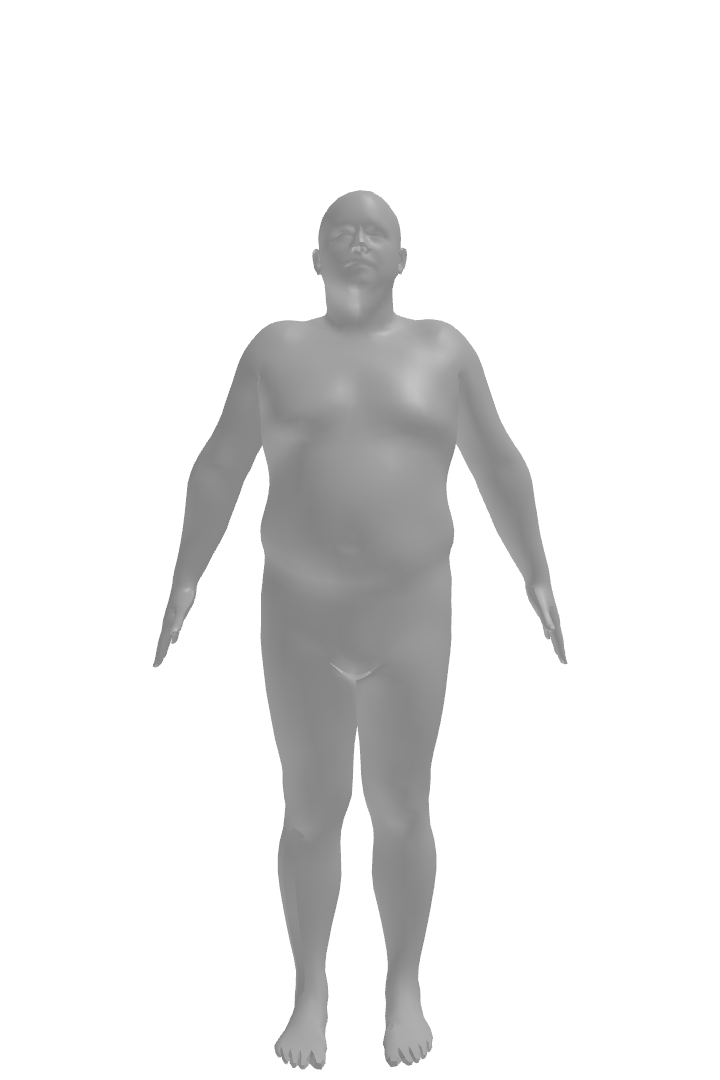
\includegraphics[width=75pt]{files/patient_8/8_2}
	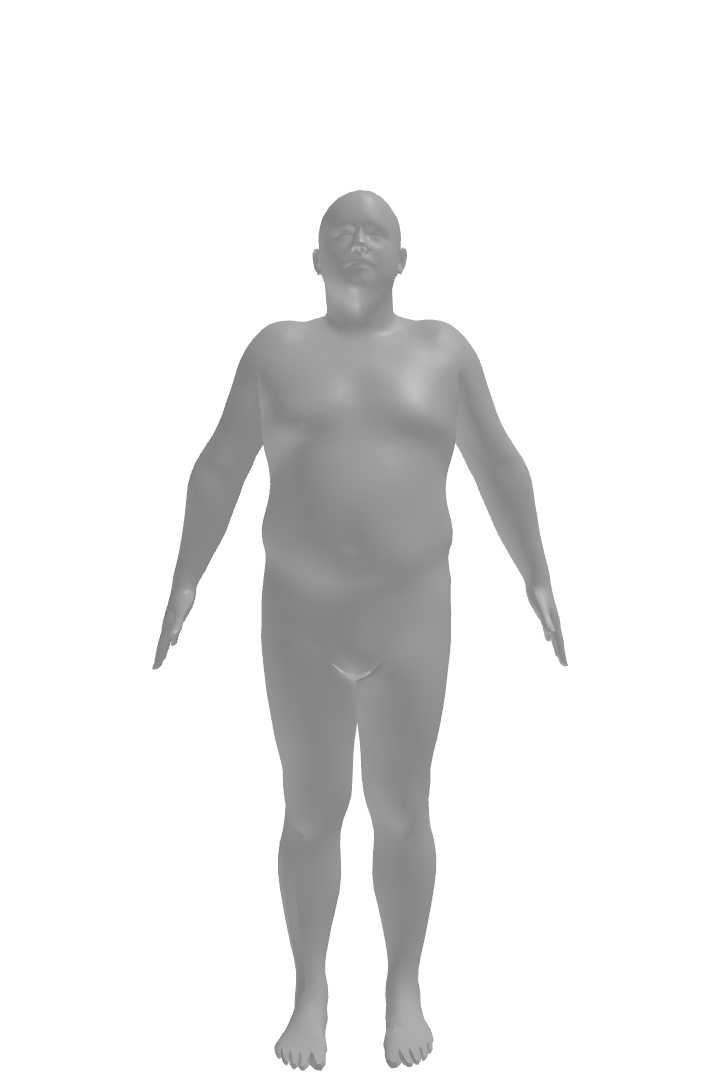
\includegraphics[width=75pt]{files/patient_8/8_3}
	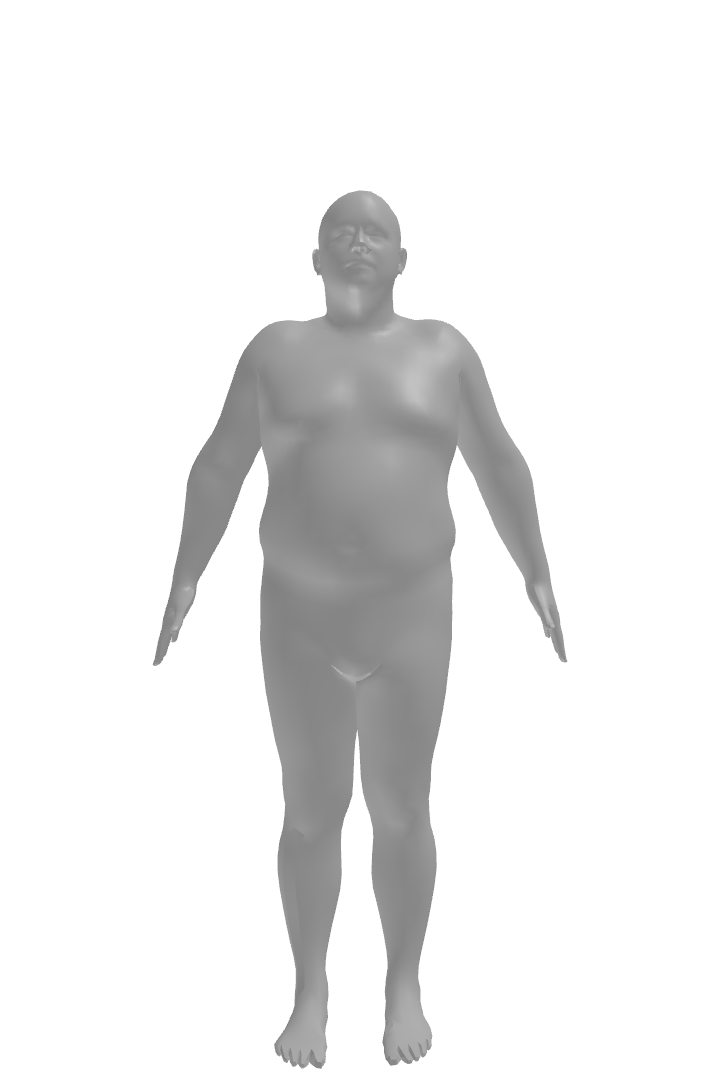
\includegraphics[width=75pt]{files/patient_8/8_4}
	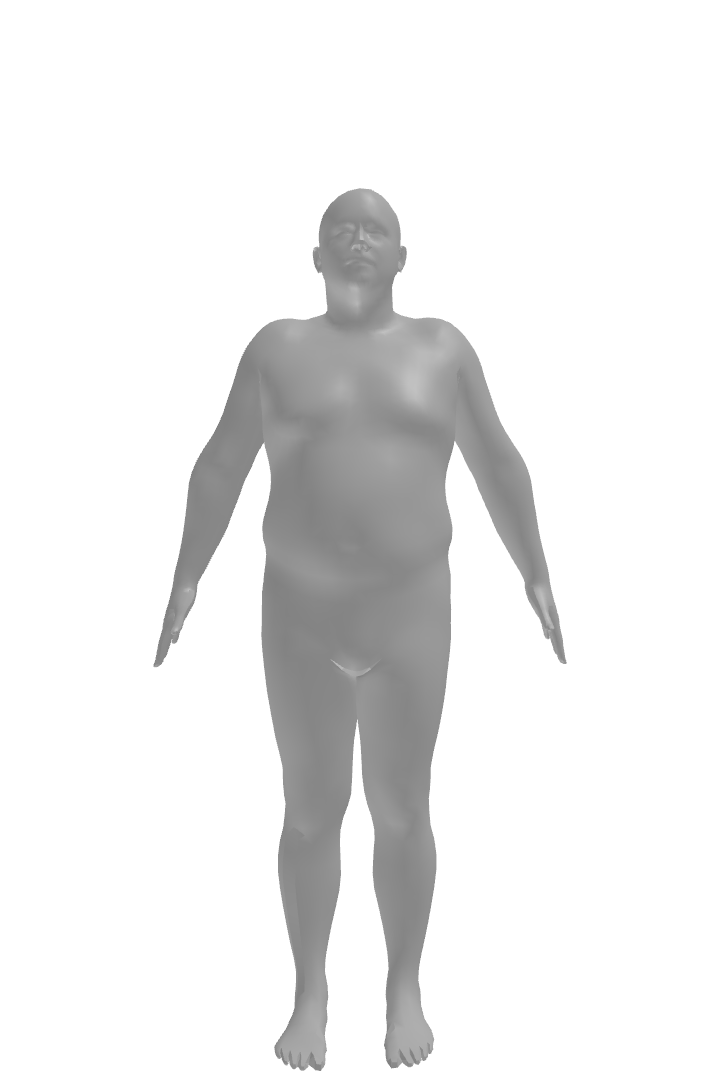
\includegraphics[width=75pt]{files/patient_8/8_5}
	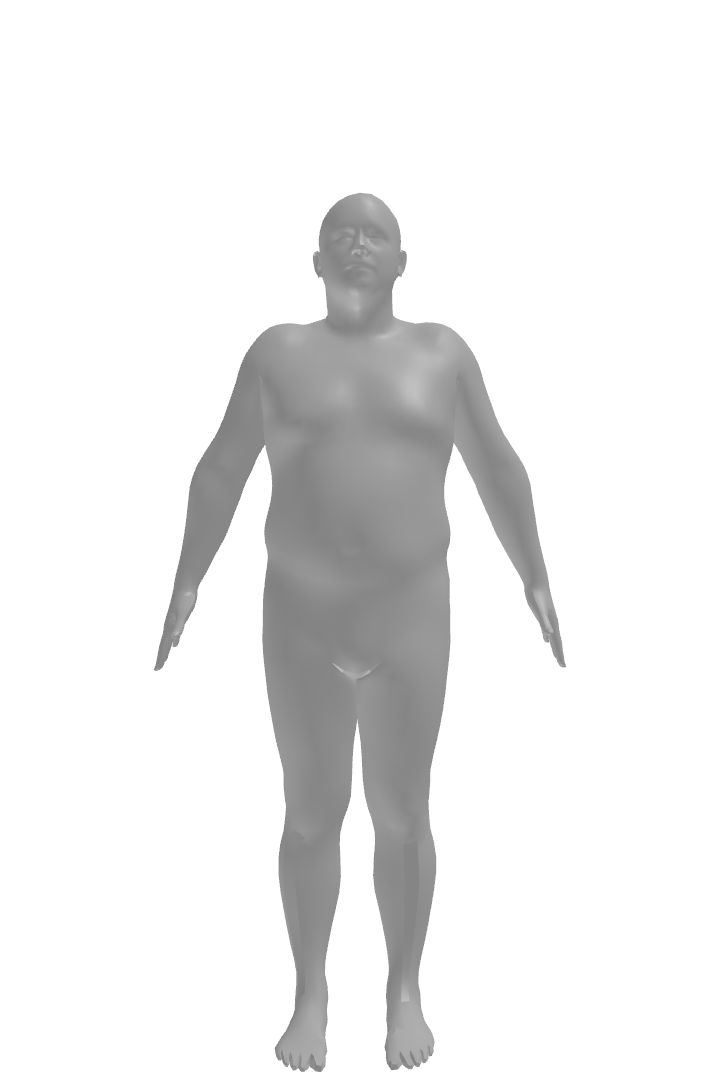
\includegraphics[width=75pt]{files/patient_8/8_6}
	\caption[Reconstructed 3D body of a patient's scans]{3D model reconstruction of a patient's body at different stages of a weight loss
		treatment. There is around a month between each scan, and a total
		weight loss of 3.8 kg.}
\end{figure}

Besides body scans, the study also collected other medical data, including
variables such as weight, localized fat and muscle mass, activity levels and
other psychological factors.

Subsequently, we wondered if it would be feasible to utilize the datasets
acquired in this prior study to formulate a predictive model. This model would
project anticipated changes in a person's body undergoing weight loss treatment
before the treatment concludes, further bolstering adherence to the treatment
regimen.

The present work explores the development of such a model. This includes
analyzing data from the earlier study, reviewing existing techniques in human
body model representation, encoding patient data using the chosen
representation, devising a neural network architecture for predicting patient
body changes, training and evaluating the model and finally, generating 3D
meshes of the predicted body changes.

We will expand on the details of this process in the following chapters.
Chapter \nameref{chap:data} will delve into the data collected during the
previous study, and how we processed it to prepare it for use in our model, as
well as how we encoded the human body scans. Afterwards, chapter
\nameref{chap:nn} will go over the neural network architecture we devised for
this project, as well as the training process and the results obtained.
Finally, chapter \nameref{chap:results} will discuss the results of our model,
and chapter \nameref{chap:conclusion} will conclude the document with a summary
of the work done and possible future lines of research.

\section{Background}

As previously mentioned, this section will provide a brief overview of the
\gls{sota} in the field of human body representation and generative neural
network architectures. We were able to use what we learned from the research on
3D human body models to write and submit a paper to the \gls{iwann} 2023
conference. \todo{link}

\subsection{3D human body representation}

The field of 3D human body recovery has seen a significant advancement with the
development of parametric models. These methods use a set of parameters to
represent body shape and pose and are widely used for reconstructing 3D human
body. These methods have different features, with some focusing on body
deformations, others on shape and pose optimization, and others on the
separation of body shape into identity-specific and pose-dependent components,
among other things. The advancements in the field have led to improved accuracy
and stability in representing human body shapes and poses. On the other hand,
in recent years various generative methods have been developed to generate 3D
models of the human body. Variational Autoencoder (VAEs) and Generative
Adversarial Networks (GANs) are two commonly used types of neural networks for
this purpose. These methods can generate 3D human body models by learning the
distribution of the data. There are many areas that can make use of these
models. Some of the most significant applications include:

\begin{itemize}
	\item Medicine: Human body models are valuable in the study of
	      anatomy~\cite{https://doi.org/10.1002/ase.1718} and for patient monitoring.
	\item Film industry: Human body models can be used to capture motion data and render
	      high-quality CGI humans.
	\item Video game industry: Human body models can be used to create realistic
	      animations and interactions between characters\cite{Starke2021}.
	\item Extended reality: Human body models can be used to capture user input in
	      virtual reality as well as rendering realistic characters.
	\item Clothing: These models can be used for fitting virtual
	      clothes\cite{apeagyei2010application} and creating realistic images of clothing
	      products.
\end{itemize}

A straightforward approach to categorize human body representations is to
classify based on the required input type and the generated output.

Regarding input, representations fall into three categories:

\begin{itemize}
	\item 2D input: These representations utilize 2D images or videos as input.
	      Some models may also process images from varying angles. The flexibility
	      of these models is beneficial as they do not necessitate specific hardware
	      to capture the input data.
	\item 3D input: Typically, these models require 3D point clouds as input data.
	\item Parametric models: These models demand a set of parameters describing the body.
	      Some models categorize these parameters into body shape and body pose. This
	      form of representation is highly intriguing for machine learning applications
	      due to the significant reduction in input data dimensionality. This factor
	      permits the training of a neural network with fewer samples. However, it
	      necessitates a model capable of generating parameters from the input data.
\end{itemize}

Some of the most common 3D output types are:

\begin{itemize}
	\item 3D meshes: These models create a 3D mesh of the object.
	\item 3D voxel: These models produce a 3D voxel grid of the object.
	      However, this approach is not widespread as it is generally not
	      beneficial for most applications.
	\item \gls{nerf}: This novel 3D representation directly renders the object
	      from a specific viewpoint. While this allows for the generation of
	      highly realistic images, it proves less beneficial for applications
	      requiring a true 3D representation of the object.
\end{itemize}

\subsubsection{Generation}

When it comes to generating 3D human models, we distinguish two main
approaches. The first approach is to use a general purpose generator system and
guide it to generate human models. The second approach is to use a generator
that has been specifically designed to generate human models from the start.

\paragraph{Human specific}

SiCloPe \cite{SiCloPe} models clothed human bodies using deep generative
models. It can reconstruct a complete and textured 3D model of a person wearing
clothes from a single input picture. It uses a silhouette-based representation
that combines 2D silhouettes and 3D joints of a body pose to describe the
complex shape variations of clothed people. It synthesizes consistent
silhouettes and feeds them into a deep visual hull algorithm for 3D shape
prediction and uses a conditional generative adversarial network to infer the
texture of the subject's back view.

PIFu \cite{PIFu} is a highly effective implicit representation that locally
aligns pixels of 2D images with their corresponding 3D object. The method can
infer 3D surface and texture from a single image or multiple input images. It
can handle intricate shapes and their variations and deformations, and can
produce high-resolution surfaces including largely unseen regions such as the
back of a person. It extends naturally to arbitrary number of views and is
memory efficient, spatially aligned with the input image and can handle
arbitrary topology. PIFuHD \cite{PIFuHD} builds on top of PIFu with an
additional module and applies it to the task of human digitalization.

Tex2Shape \cite{Tex2Shape} is a simple method to infer detailed full human body
shape from a single photograph. It turns shape regression into an aligned
image-to-image translation problem and estimates detailed normal and vector
displacement maps from partial texture maps of the visible region. The results
feature details even on parts that are occluded in the input image and the
model generalizes well to real-world photographs.

HumanMeshNet \cite{HumanMeshNet} regresses a template mesh's vertices and
receives regularization from 3D skeletal locations in a multi-branch,
multi-task framework. It focuses on implicitly learning the mesh representation
and is a novel model for 3D human body reconstruction from a monocular image.

DeepHuman \cite{DeepHuman} is image-guided 3D human reconstruction network that
leverages a dense semantic representation and fuses different scales of image
features into the 3D space. The visible surface details are refined through a
normal refinement network. The method outperforms state-of-the-art approaches
in 3D human model estimation from a single image.

HumanGen \cite{humangen} is a 3D human generation scheme with detailed geometry
and 360° realistic free-view rendering. The scheme marries the 3D human
generation with various priors from the 2D generator and 3D reconstructor of
humans through the design of an "anchor image." The authors adopt a pronged
design to disentangle the generation of geometry and appearance and use an
anchor image to adapt a 3D reconstructor for fine-grained details synthesis and
propose a two-stage generation scheme for geometry and appearance.

HumanNeRF \cite{humannerf} describes a neural representation for high-fidelity
free-view synthesis of dynamic humans. It uses an aggregated pixel-alignment
feature with a pose embedded non-rigid deformation field and raw HumanNeRF can
already produce reasonable rendering on sparse video inputs. The approach is
improved with in-hour scene-specific fine-tuning and appearance blending. The
authors show that this approach is effective in synthesizing photorealistic
free-view humans with sparse camera view inputs.

\paragraph{General}

The CoCosNet \cite{CoCosNet} (and CoCosNet v2 \cite{CoCosNet2}) paper
introduces full-resolution correspondence learning for cross-domain image
translation. It uses a hierarchical strategy that employs the correspondence
from coarse to fine levels and utilizes the ConvGRU module to refine the
current correspondence. The result is a highly efficient and effective approach
for exemplar-based image translation that outperforms state-of-the-art
literature.

\subsubsection{Generative neural networks}

\section{Objectives}\label{objectives}

\begin{itemize}
	\item \textbf{Objective 1} Study the state of the art in human body representation and
	      generation. \subitem Review the literature on human body representation and
	      generation. \subitem Analyze the advantages and disadvantages of the different
	      approaches. \subitem Select the most suitable approach for the project.
	\item \textbf{Objective 2} Analyze and process the data to be used in the project. \subitem
	      Explore the data and its characteristics. \subitem Preprocess the data to be
	      used in the project, identifying and solving any issues that may arise.
	      \subitem Study what data augmentation techniques can be applied to the data.
	\item \textbf{Objective 3} Design and implement a neural network that can understand human
	      bodies and train it to predict shape changes in time. \subitem Study the
	      different neural network architectures that can be used in a time series
	      prediction problem. \subitem Design a neural network architecture that can be
	      used to generate future human body shapes. \subitem Implement the neural
	      network architecture. \subitem Train the neural network. \subitem Evaluate the
	      predictions made by the neural network.
	\item \textbf{Objective 4} Evaluate the results. \subitem Generate predicted human body
	      shapes for a set of input data. \subitem Evaluate the predictions.
\end{itemize}


\chapter{Data Analysis and Preprocessing}\label{chap:data}

As we mentioned in Chapter \ref{chap:introduction}, our work is based on a
dataset collected for a study on the effects of visualizing the progress of
weight loss using a \gls{vr} headset during a weight loss treatment.

\section{3D body model dataset under dietetic treatment}

Our dataset comprises approximately 400 sessions obtained from 80 distinct
patients. These sessions, recorded at irregular intervals, incorporate a 3D
scan of the patient and a multitude of other measurements such as weight,
height, body fat percentage, and more.

\begin{table}[h]
	\centering
	\begin{tabular}{ l l l }
		\toprule
		Type                               & Source                                                                                         & Measurement (unit)                        \\
		\midrule
		\multirow{3}{*}{Anthropometric}    & \multirow{3}{4cm}{Flexible measuring tape}                                                     & Wrist (cm)                                \\
		                                   &                                                                                                & Waist (cm)                                \\
		                                   &                                                                                                & Hip (cm)                                  \\
		\midrule

		\multirow{6}{*}{Body composition}  & \multirow{6}{4cm}{Tanita\textregistered\ MC 780-P MA and Seca\textregistered\ 213 stadiometer} & Fat per limb and trunk (\%)               \\
		                                   &                                                                                                & Muscle per limb and trunk (\%)            \\
		                                   &                                                                                                & Total fat and muscle (\%)                 \\
		                                   &                                                                                                & Visceral fat area (cm\textsuperscript{2}) \\
		                                   &                                                                                                & Weight (kg)                               \\
		                                   &                                                                                                & Height (m)                                \\
		\midrule

		\multirow{3}{*}{Other, Lifestyle}  & \multirow{3}{4cm}{Interview}                                                                   & Activity   (score)                        \\
		                                   &                                                                                                & Gender                                    \\
		                                   &                                                                                                & Age (years)                               \\

		\midrule

		\multirow{3}{*}{Blood (capillary)} & \multirow{3}{4cm}{Accutrend\textregistered\ Plus}                                              & Glucose (mg/dL)                           \\
		                                   &                                                                                                & Cholesterol (mg/dL)                       \\
		                                   &                                                                                                & Triglycerides (mg/dL)                     \\

		\midrule

		\multirow{2}{*}{Blood pressure}    & \multirow{2}{4cm}{Omron\textregistered\ M3}                                                    & Systolic pressure (mmHg)                  \\
		                                   &

		                                   & Diastolic pressure (mmHg)                                                                                                                  \\
		\bottomrule

	\end{tabular}
	\caption{Measurements collected from each session \citep{10045_124160}.}
\end{table}

The raw data, however, required extensive cleaning before it could be analyzed.
We encountered sessions missing certain measurements and numerous data
outliers. After our data cleaning process, we were left with approximately 200
viable sessions.

\begin{figure}[h]
	\centering
	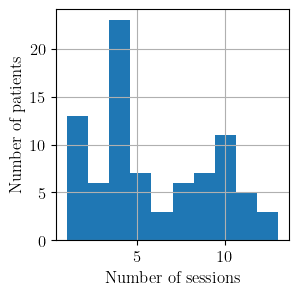
\includegraphics{files/sessions_per_patient}
	\caption{Variation in the number of sessions per patient.}
	\label{fig:sessions-per-patient}
\end{figure}

As Figure~\ref{fig:sessions-per-patient} illustrates, the number of sessions
per patient varied significantly, with some patients attending only a single
session and others attending over ten. Given that neural networks necessitate
uniform input shapes, we were faced with a challenge. We'll elaborate on how we
tackled this problem in Chapter \ref{chap:nn}.

\section{Data Cleaning and Outlier Detection}

A data cleaning pipeline was constructed utilizing the \gls{pandas} library.
The essential steps involved in the data cleaning process included missing data
treatment, invalid data removal, and variable unit standardization.

We indexed our dataset with a multi-index that included the patient's id and
the session number. This system facilitated patient-specific data iteration and
simplified the process of pinpointing patient data discrepancies.

Upon scrutinizing plotted data, we discovered that the decimal separator was a
common source of errors. Many measurements appeared to be inflated by a factor
of 10, prompting us to devise tailored rules to correct this. Additional rules
were implemented to identify and discard out-of-range values or those
conflicting with other measurements. These rules included:

\begin{itemize}
	\item Small variation between measurements of different limbs, such as muscle or fat
	      percentage discrepancies between left and right arms.
	\item Ensuring that the combined muscle and fat percentages do not exceed 100\%.
	\item Verifying that the fat and muscle percentage levels individually stay below
	      100\% --- values exceeding this typically indicate a measurement inflated by a
	      factor of 10.
\end{itemize}

Despite these rectifications, some outliers persisted. We experimented with a
system that flagged dramatic session-to-session changes, but found it too
susceptible to false positives. Eventually, we opted to manually inspect the
data, flagging conspicuous outliers for removal.

\begin{figure}[h]
	\centering
	\begin{subfigure}{\textwidth}
		\centering
		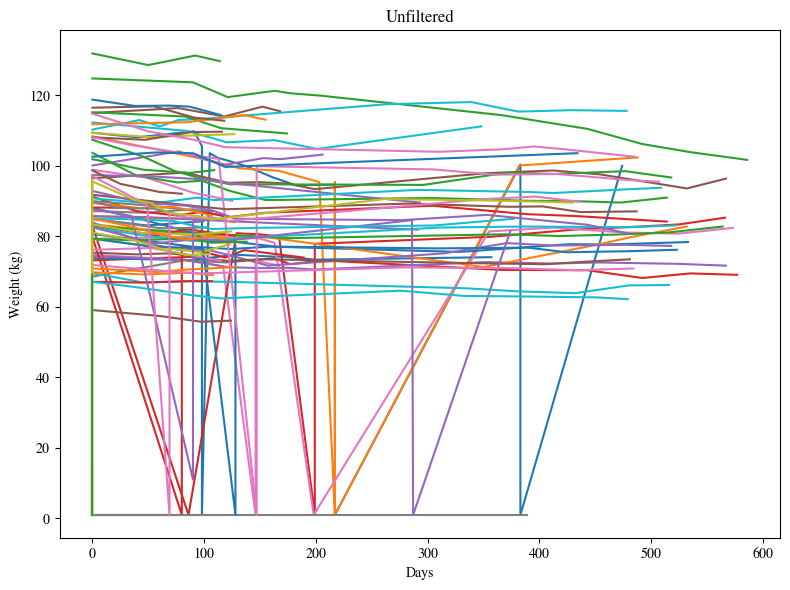
\includegraphics[width=0.8\textwidth]{files/weight_unfiltered}
		\caption{Raw weight.}
	\end{subfigure}
	\begin{subfigure}{\textwidth}
		\centering
		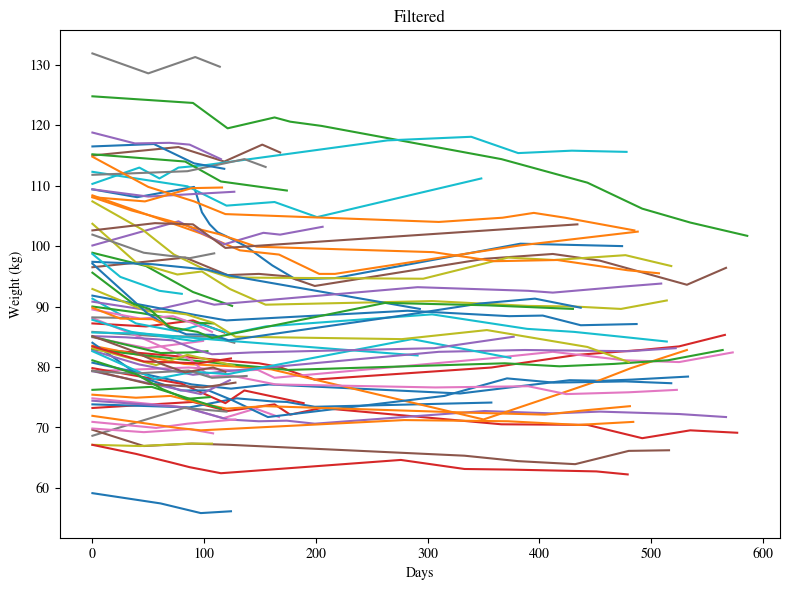
\includegraphics[width=0.8\textwidth]{files/weight_filtered}
		\caption{Filtered weight.}
	\end{subfigure}
	\caption{Weight measurements pre and post filtering.}
\end{figure}

\section{SMPL for Body Representation}

In our study, we found it crucial to accurately represent the human body's
complex and varied structure. This necessity led us to adopt the \gls{smpl}
model. \gls{smpl} is a versatile and practical mathematical model for capturing
a wide range of human body shapes and poses. It provides a parametric approach
to represent the body shape and pose in a low-dimensional linear space, thus
making it a valuable asset in our research.

\gls{smpl} characterizes the human body using two sets of parameters: shape ($\beta$)
and pose ($\theta$). The shape parameters ($\beta$) are derived from a
principal component analysis of the shapes in a training set. \gls{smpl} uses a
vector of 10 shape coefficients that define the primary modes of shape
variation. These coefficients cover a wide array of human body shapes, allowing
us to capture a comprehensive view of a patient's body structure.

\begin{figure}[H]
	\centering
	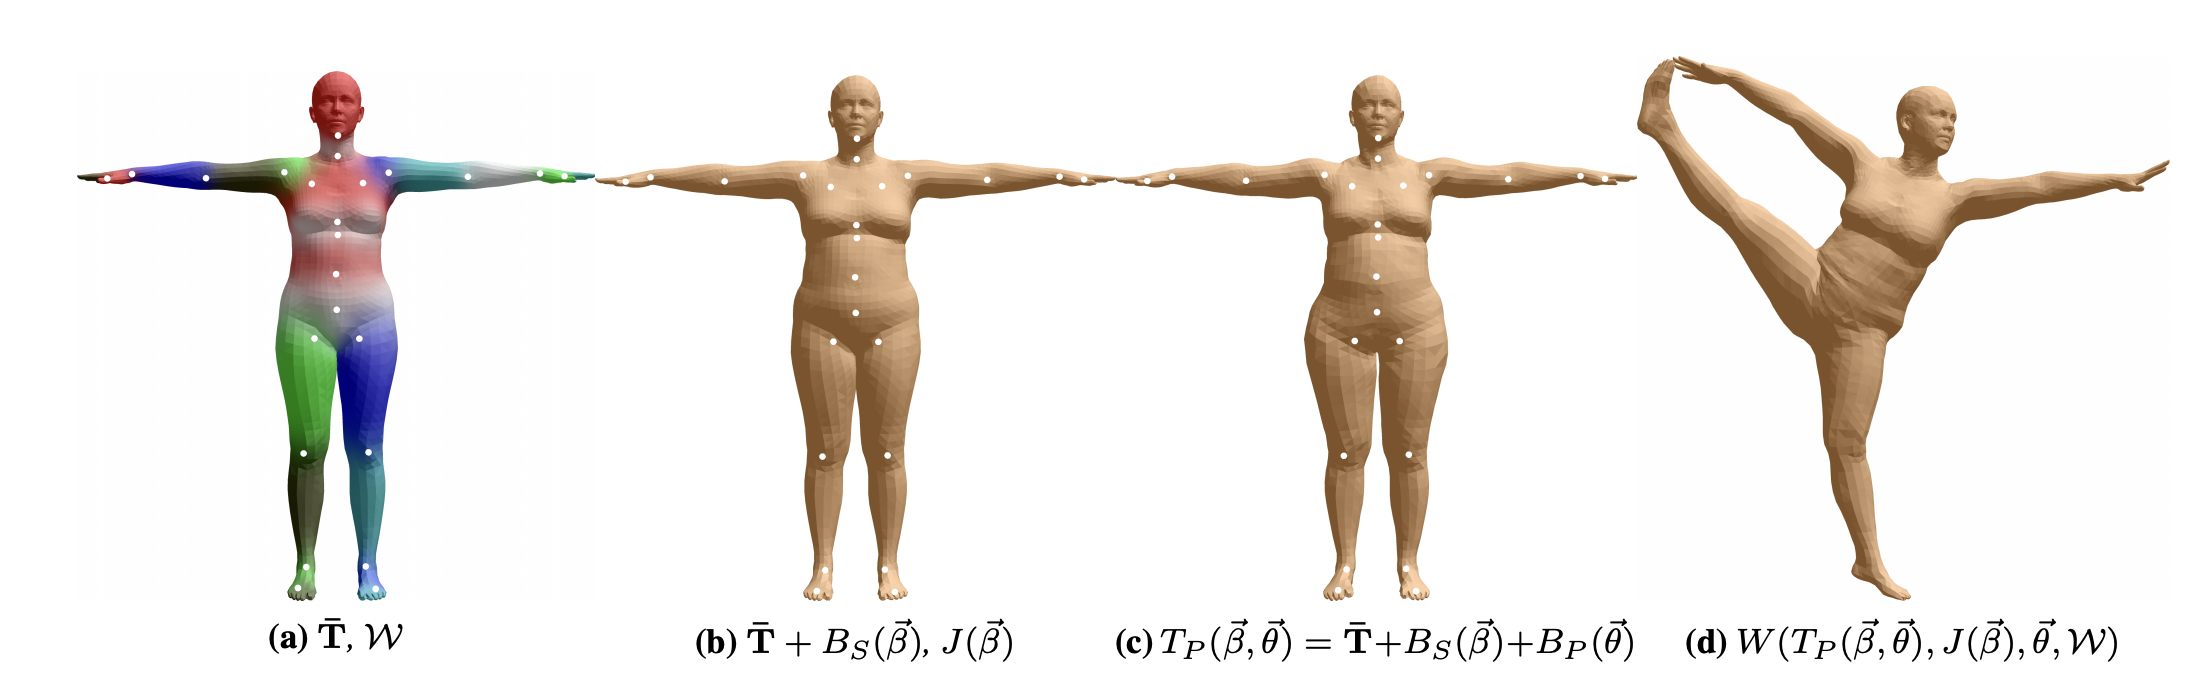
\includegraphics[width=\textwidth]{files/SMPL_formulation}
	\caption{SMPL model \citep{meshcapade}}
	\label{fig:SMPL_formulation}
\end{figure}

On the other hand, the pose parameters ($\theta$) represent the orientation of
the body's joints. This parameter encodes the body's pose into 72 pose
coefficients. While the pose parameters offer a detailed portrayal of body
position, our interest primarily lies in the body shape. Therefore, we focus on
the shape parameters for our study.

\gls{smpl} serves as an ideal fit for our problem due to its compact, continuous, and
differentiable nature. The model's low-dimensionality reduces computational
complexity, making it a practical choice for large-scale analysis. Moreover,
the differentiable nature of the model facilitates gradient-based optimization
methods, essential for precise parameter estimation. The model's continuous
representation also allows for a seamless transition between different body
shapes, further enhancing the realism and accuracy of the body representations.

We extracted \gls{smpl} parameters — shape ($\beta$) and pose ($\theta$) — from
the 3D scans using a custom minimization algorithm \citep{estimation:2023}.
This method encompassed the following stages:

\begin{figure}[H]
	\centering
	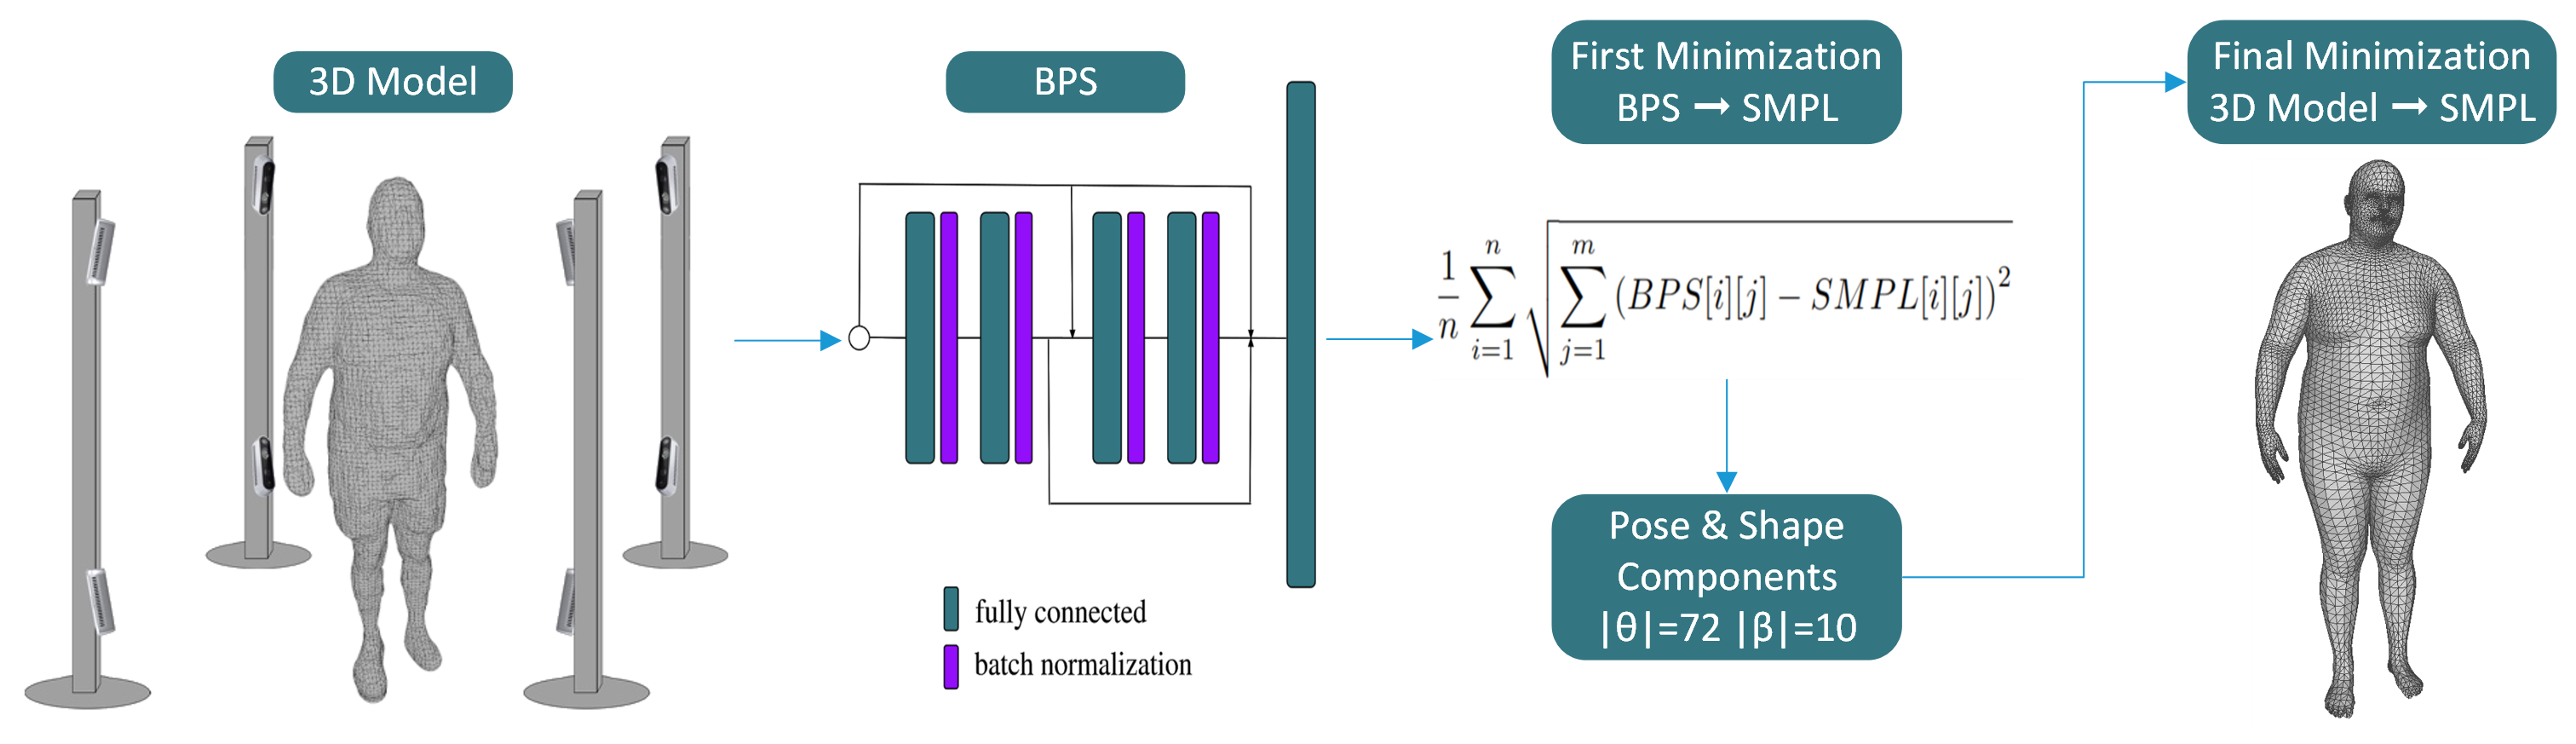
\includegraphics[width=\textwidth]{files/pipeline_smpl.png}
	\caption{Our pipeline for extracting SMPL parameters from 3D scans.}
\end{figure}

\begin{itemize}
	\item Acquiring and Preprocessing of 3D Data: The Tech4Diet project's system, fitted
	      with 13 Intel RealSense RGB-D cameras, was used to capture the 3D data (Figure
	      \ref{fig:cameras_scan}). This data was then preprocessed to minimize noise and
	      optimize 3D scan alignment.

	\item Estimating an Intermediate Template using a BPS Neural Network: The \gls{bps}
	      method was used to generate an intermediate 3D model by encoding a set of
	      points into fixed-distance representations. A DenseNet neural network then took
	      this \gls{bps} representation as input to predict the vertex positions of a
	      template resembling the input point cloud.

	\item First Minimization: \gls{bps} to \gls{smpl}: We minimized the pose and shape
	      parameters of the \gls{smpl} model to align it with the template created by the
	      \gls{bps}.

	\item Second Minimization: 3D Scan to \gls{smpl}: A second minimization was performed
	      to align the \gls{smpl} model with the 3D scan from the RGB-D sensors. We
	      proposed an algorithm to enhance the speed and accuracy of this process by
	      segmenting the model into body parts, applying rigid registration, and then
	      using a custom minimization function that considered both distance and normal
	      angles.
\end{itemize}

\begin{figure}[H]
	\centering
	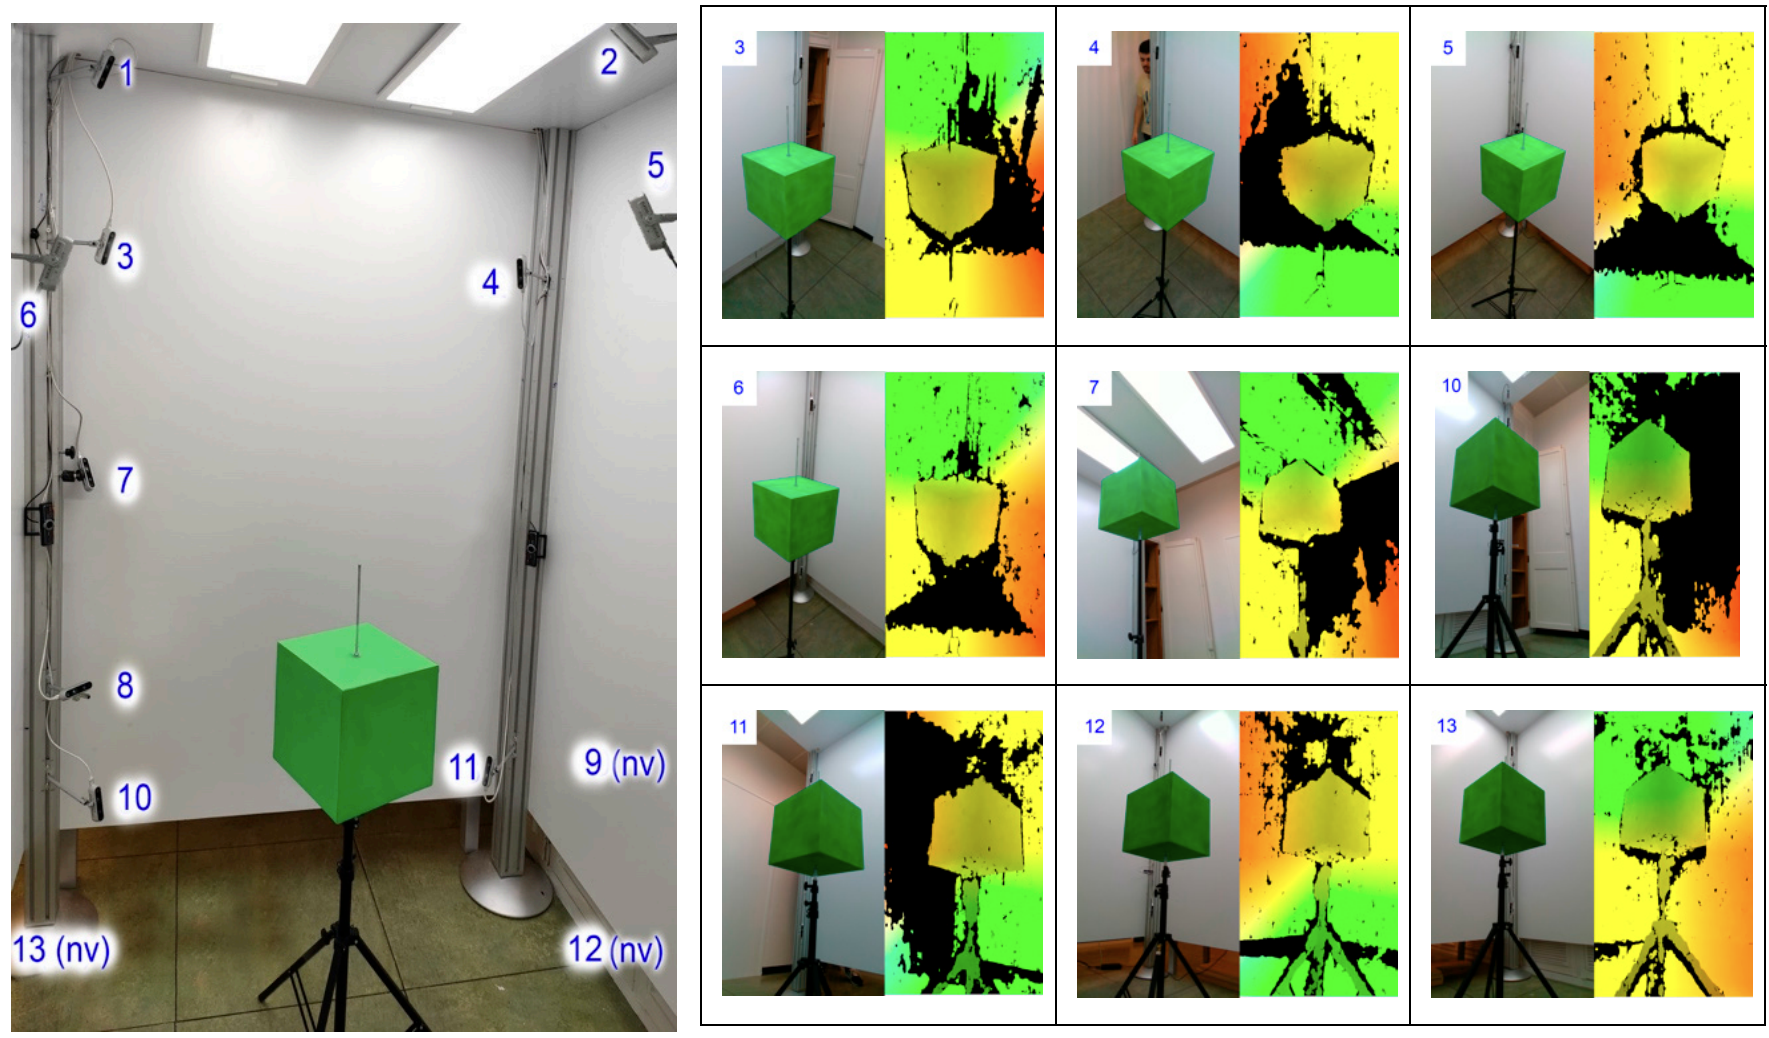
\includegraphics[width=\textwidth]{files/cameras_scan.png}
	\caption{Our 3D scanning system.}
	\label{fig:cameras_scan}
\end{figure}

Figures \ref{fig:beta-1-vis} to \ref{fig:beta-10-vis} (in the Annex
\ref{chap:annex1}) demonstrate the effects of shape parameter variations.
Although we employed a scale of 3 to amplify their effects for visualization,
actual values are significantly lower. $\beta_1$ regulates the overall body
height, while $\beta_2$ is highly correlated with the body mass index.

\begin{table}[h]
	\centering
	\begin{tabular}{c | c c c c c c c c c c}
		\toprule
		     & $\beta_1$ & $\beta_2$ & $\beta_3$ & $\beta_4$ & $\beta_5$ & $\beta_6$ & $\beta_7$ & $\beta_8$ & $\beta_9$ & $\beta_{10}$ \\
		\midrule
		mean & 0.88      & -0.73     & 0.34      & 0.01      & 0.06      & 0.06      & 0.11      & 0.02      & 0.01      & 0.11         \\

		std  & 0.97      & 0.78      & 0.26      & 0.21      & 0.12      & 0.13      & 0.08      & 0.03      & 0.03      & 0.08         \\

		min  & -1.42     & -2.57     & -0.64     & -0.65     & -0.23     & -0.25     & -0.14     & -0.07     & -0.08     &
		-0.17                                                                                                                           \\

		25\% & 0.12      & -1.26     & 0.15      & -0.14     & -0.01     & -0.02     & 0.04      & 0.00      & -0.01     & 0.06         \\

		50\% & 0.94      & -0.69     & 0.36      & 0.03      & 0.04      & 0.02      & 0.11      & 0.02      & 0.01      & 0.11         \\

		75\% & 1.66      & -0.20     & 0.52      & 0.17      & 0.14      & 0.14      & 0.16      & 0.04      & 0.04      & 0.17         \\

		max  & 2.90      & 2.96      & 0.97      & 0.45      & 0.39      & 0.47      & 0.36      & 0.13      & 0.16      & 0.30         \\
		\bottomrule
	\end{tabular}
	\caption{Statistics of the shape parameters.}
\end{table}

\section{Exploring Additional Datasets}

Finding the right data is like searching for a needle in a haystack. It's a key
task if we want to improve our model, but it's also quite a challenge - and for
us, it was even more so due to a few reasons.

First, a lot of medical data isn't exactly out there for anyone to pick up and
use. Understandably, these datasets are kept private due to concerns around
confidentiality and privacy, which are of utmost importance when it comes to
health-related data. This makes these datasets not only hard to come by, but
also tough to gauge in terms of their usefulness for our work. It's hard to
tell if a dataset is going to be helpful if we can't even get a peek at what's
inside.

Second, there are open-source datasets with 3D scans of people. But there's a
catch: these datasets usually only provide a snapshot of a person's physique at
one point in time. They don't show how a person's body changes over time, which
is a key piece of the puzzle in our study on how diet interventions affect body
shape.

We also looked at datasets from fields like sports science or anthropometry.
These weren't specifically designed for studying body composition, but we
thought they might still have some useful data. However, the scope of the data,
the level of detail, and the lack of consistent body composition measurements
meant that these datasets didn't quite fit the bill either.

Considering these challenges, we decided to use our own data for training and
testing our model. To get around the limitations of our data, we looked into
techniques to artificially expand our dataset. We'll talk more about how we did
this in Chapter \ref{chap:nn}.
\chapter{Neural network}\label{chap:nn}

\todo{what are neural networks and why are they useful?}

\section{Selection of Neural Network Architecture}

In light of the temporal nature of our data, we required a neural network
architecture capable of handling sequential data. Various neural network
architectures cater to this requirement. For instance, \gls{rnn} which use
outputs from previous steps as inputs for subsequent steps, excel at handling
sequential data. This trait enables \gls{rnn}s to retain information from
previous steps, a characteristic beneficial for time series analysis.

However, one downside of RNNs is the vanishing gradients problem, wherein they
tend to forget information from earlier stages in the sequence. Various
\gls{rnn} variations, such as \gls{lstm} \cite{lstm:1997} and \gls{gru}
\cite{gru:2014}, have been designed to mitigate this issue.

On the other hand, Transformer networks \cite{attention2017}, a more recent
introduction to the world of neural networks, have seen significant success in
natural language processing. These networks utilize attention mechanisms,
allowing them to concentrate on specific portions of an input sequence. While
useful for time series analysis, the major drawback of Transformer networks is
their need for vast amounts of training data\todo[]{citation needed} --- a
requirement we couldn't fulfill in this case.

Upon weighing these factors, we decided to adopt a neural network architecture
utilizing an \gls{lstm}.

\section{Neural network architecture}

Utilizing the PyTorch library, we built our custom \gls{lstm}-based neural
network architecture. \todo{what is pytorch and why did we use it?}

PyTorch's \texttt{pack\_padded\_sequence} and \texttt{pad\_packed\_sequence}
functions were used to pack and unpack sequences into
\href{https://pytorch.org/docs/stable/generated/torch.nn.utils.rnn.PackedSequence.html}{\texttt{PackedSequence}},
accommodating patients with varying numbers of sessions. An additional tensor
of \textit{lengths} was used to facilitate the input of the packed sequences
into the \gls{lstm}, which consequently ignored the values beyond the length of
the sequence.

\todo{explain more?}

\begin{figure}
    \centering
    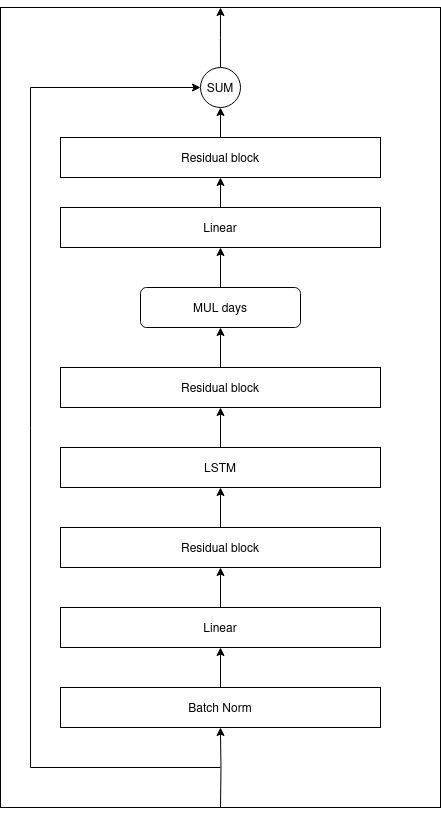
\includegraphics[width=8cm]{files/nn_diagram}
    \caption{Diagram of the implemented \gls{lstm}-based neural network architecture}
\end{figure}

\subsection{Variability in the dates of the sessions}

The dataset's sessions are not uniformly spaced in time, varying from a few
days to several months apart. This is a problem for neural networks, since they
work best with uniformly spaced data. To solve this problem, we decided to make
the neural network predict the daily change instead.

This was accomplished by adding a residual connection between the input and the
output of the neural network, and multiplying the output by the number of days
until the next session. This way, the neural network can learn to predict the
daily change, and the output is scaled to the number of days until the next
session.
\section{Training and Optimization}

During the training phase, the neural network receives input in the form of a
tensor with a shape of $(\text{batch size}, \text{max sequence length},
    \text{number of features})$, a tensor with a shape of $(\text{batch size}, 1)$
containing the length of the current sequence, and a scalar representing the
number of days until the next session. It then generates a tensor of shape
(\text{batch size}, \text{max sequence length}, \text{number of features}) that
contains the predicted values for the next session.

The neural network takes the following inputs:

\begin{itemize}
    \item A tensor of shape $(\text{batch size}, \text{max sequence length}, \text{number
                  of features})$.
    \item A tensor of shape $(\text{batch size}, 1)$ containing the length of the current
          sequence.
    \item A scalar representing the number of days until the next session.
\end{itemize}

The neural network returns:

\begin{itemize}
    \item A tensor of shape $(\text{batch size}, \text{max sequence length}, \text{number
                  of features})$ that contains the predicted values for the next session.
\end{itemize}

To construct the input features, we concatenate the $\beta$ parameters of the
\gls{smpl} model with the patient's height, weight, and age.

We also experimented with including body fat percentage and muscle mass
percentage, but the results did not show improvement, so we decided to exclude
them in order to avoid overfitting.

We utilized the AdamW optimizer with a variable learning rate and weight decay,
along with \gls{mse} loss as the objective function.

\subsection{Hyperparameter tuning}

We performed a grid search to find the optimal hyperparameters for our model.
The hyperparameters we tuned were the number of layers in the input, \gls{lstm}
and output, the number of hidden units in the \gls{lstm} and the weight decay.

The final hyperparameters we used are shown in
Table~\ref{tab:final-hyperparameters}.

\begin{table}[h]
    \centering
    \begin{tabular}{l c c}
        \toprule
        \textbf{Hyperparameter}                  & \textbf{Value} \\
        \midrule
        Number of layers in the input            & 4              \\
        Number of layers in the \gls{lstm}       & 4              \\
        Number of layers in the output           & 4              \\
        Number of hidden units in the \gls{lstm} & 32             \\
        Weight decay                             & 0.001          \\
        \bottomrule
    \end{tabular}
    \caption{Final hyperparameters used for the neural network}
    \label{tab:final-hyperparameters}
\end{table}

\section{Results}

While a more detailed analysis of the results will be presented in the next
chapter, we provide some examples of our model's predictions.

Figure \ref{fig:predicted-betas} displays the shape parameters for a patient
alongside the model's prediction.

\begin{figure}[h]
    \centering
    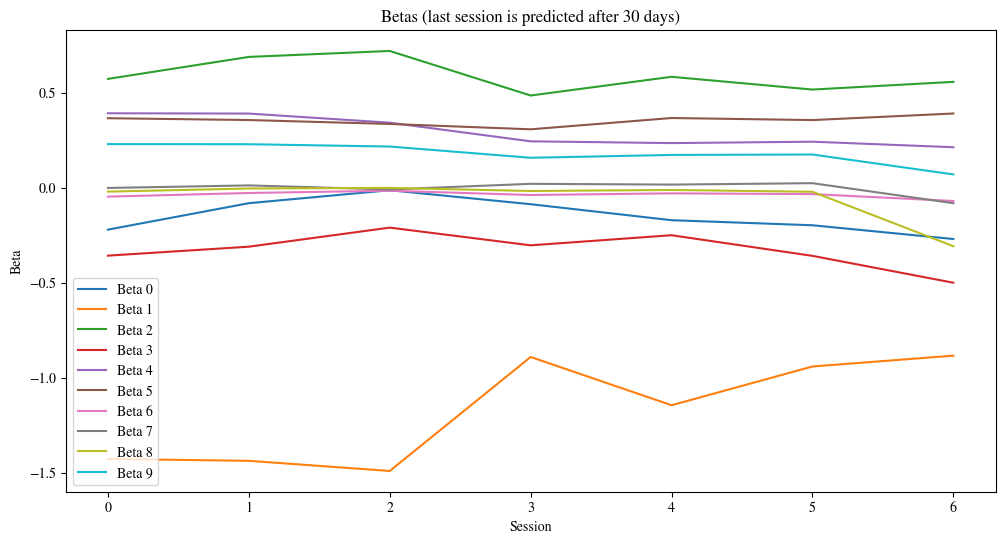
\includegraphics[width=\textwidth]{files/predicted_betas}
    \caption{Shape parameters for a patient and the model's prediction.}
    \label{fig:predicted-betas}
\end{figure}

Figure \ref{fig:patient-body-model} illustrates the reconstructed 3D model of a
patient's body, showcasing images from multiple sessions. The final image in
the sequence represents the model's prediction after one month from the last
session, with a total of 74 days between the first and last session.

\begin{figure}[h]
    \centering
    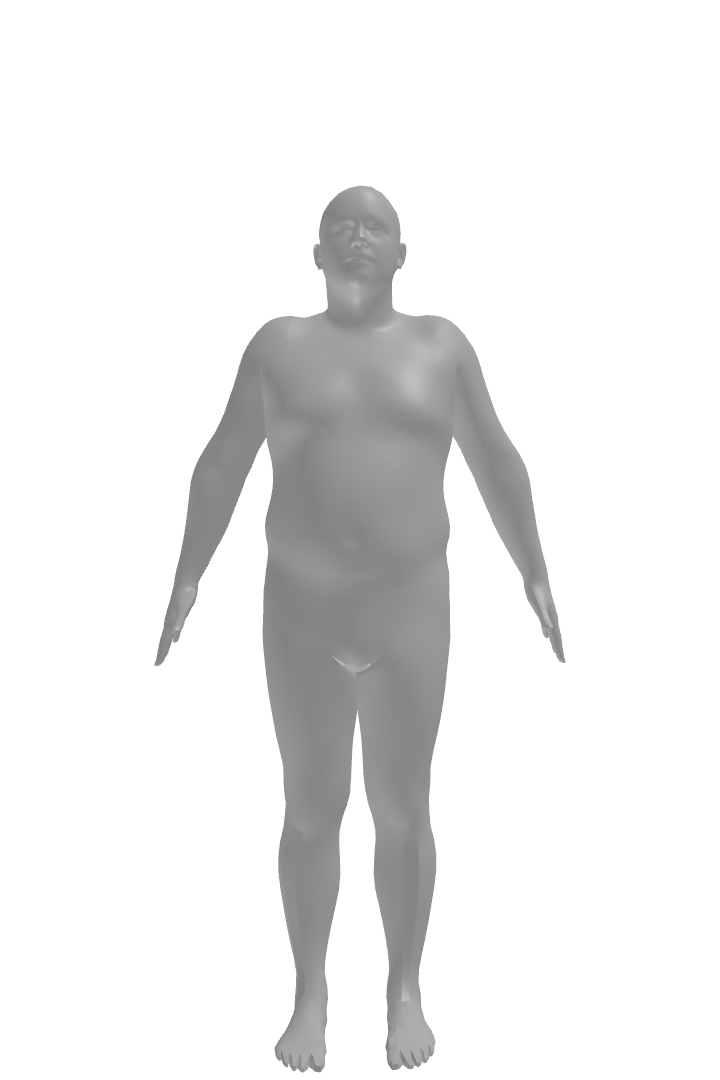
\includegraphics[width=120pt]{files/patient_2/2_6}
    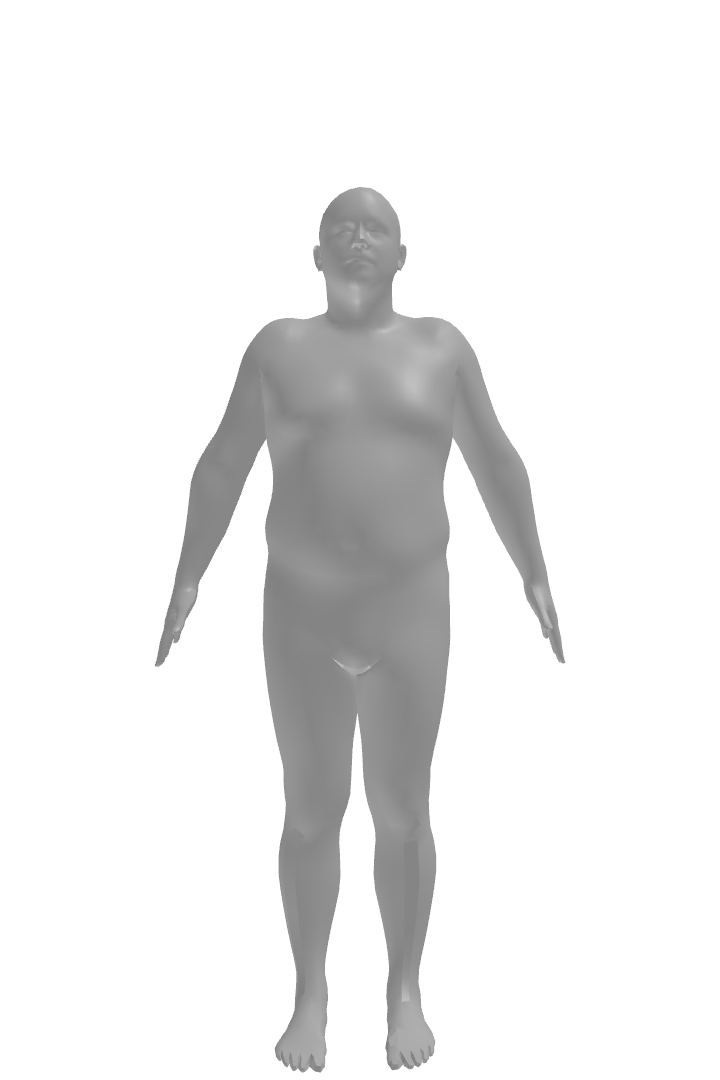
\includegraphics[width=120pt]{files/patient_2/2_7}
    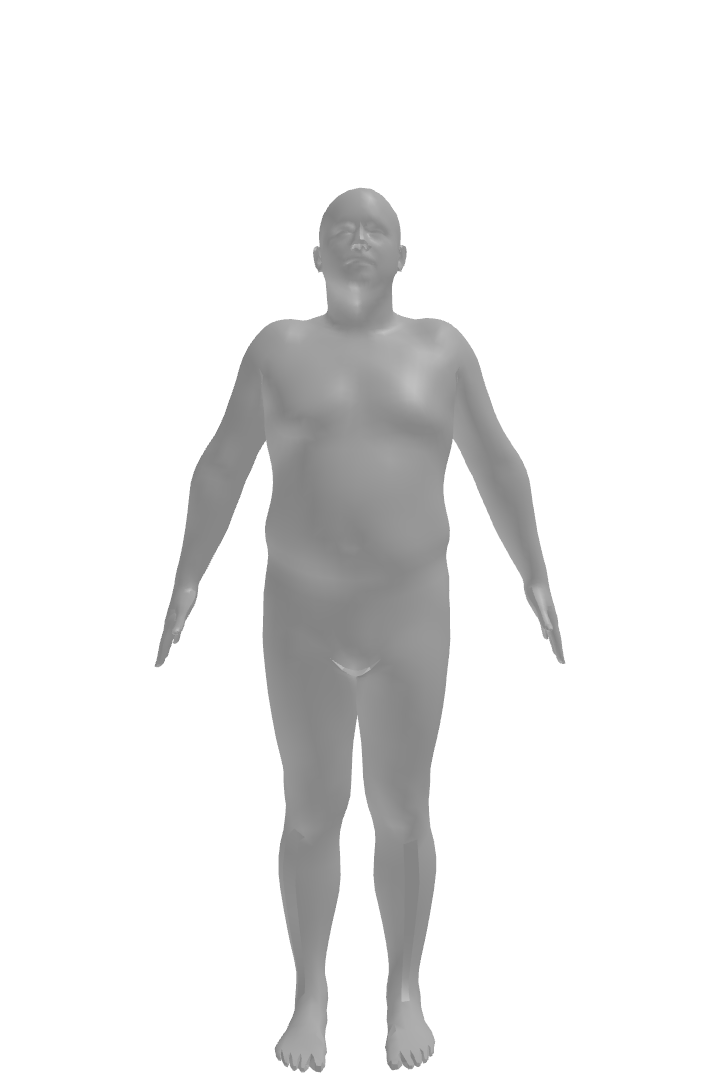
\includegraphics[width=120pt]{files/patient_2/2_8}
    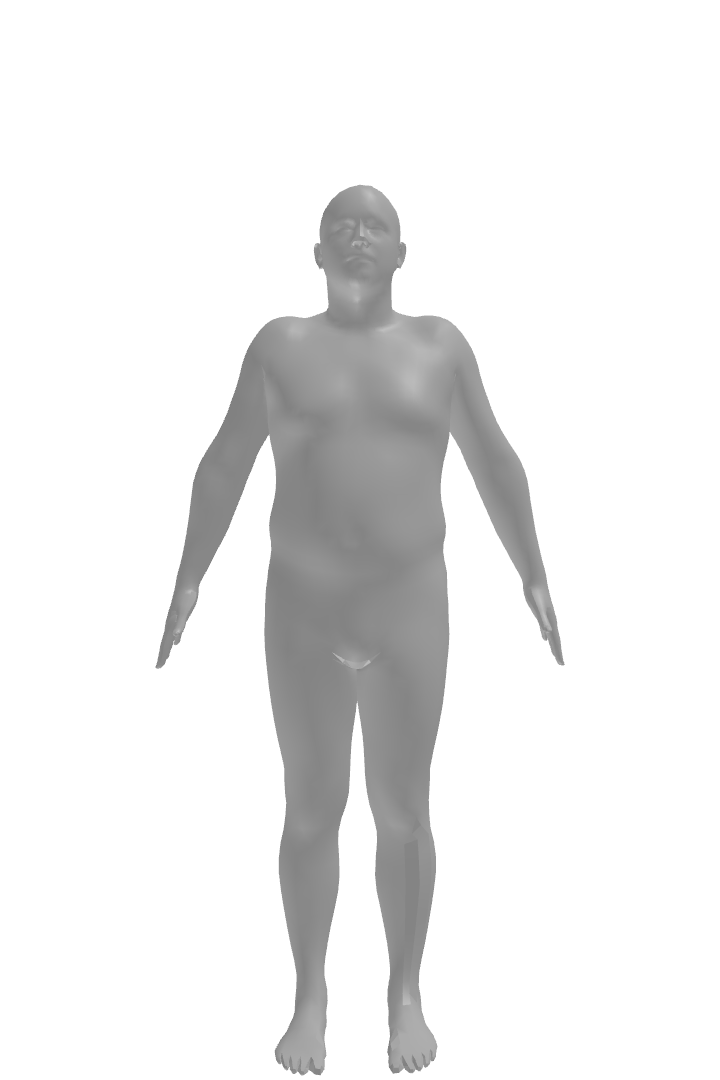
\includegraphics[width=120pt]{files/patient_2/2_9}
    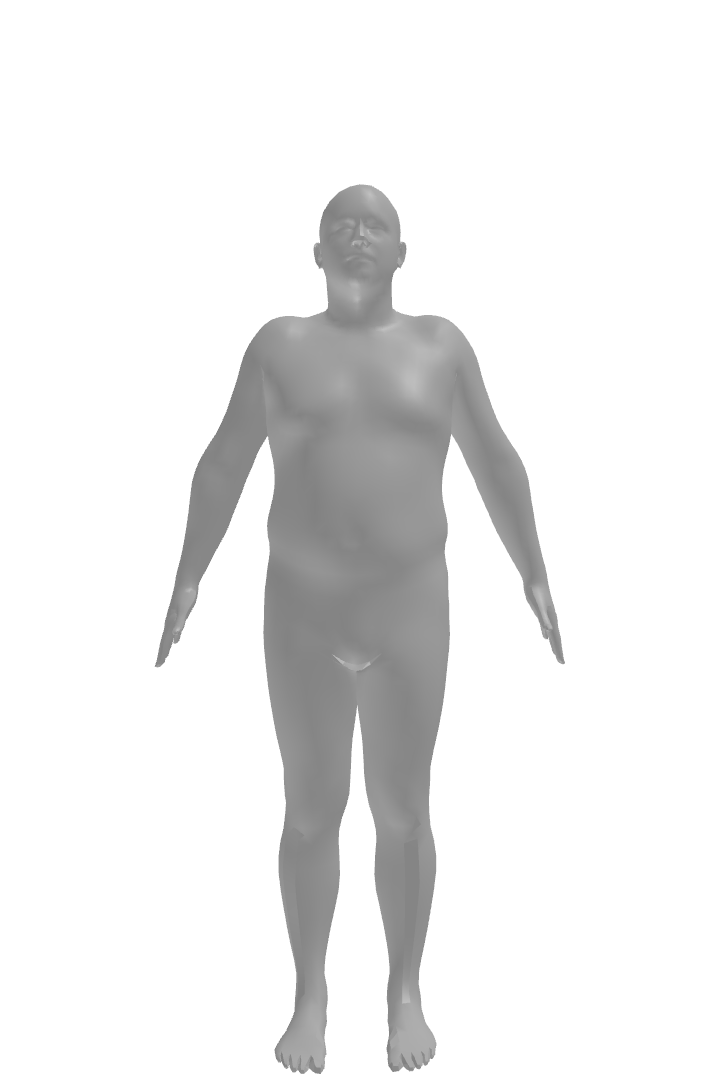
\includegraphics[width=120pt]{files/patient_2/2_10}
    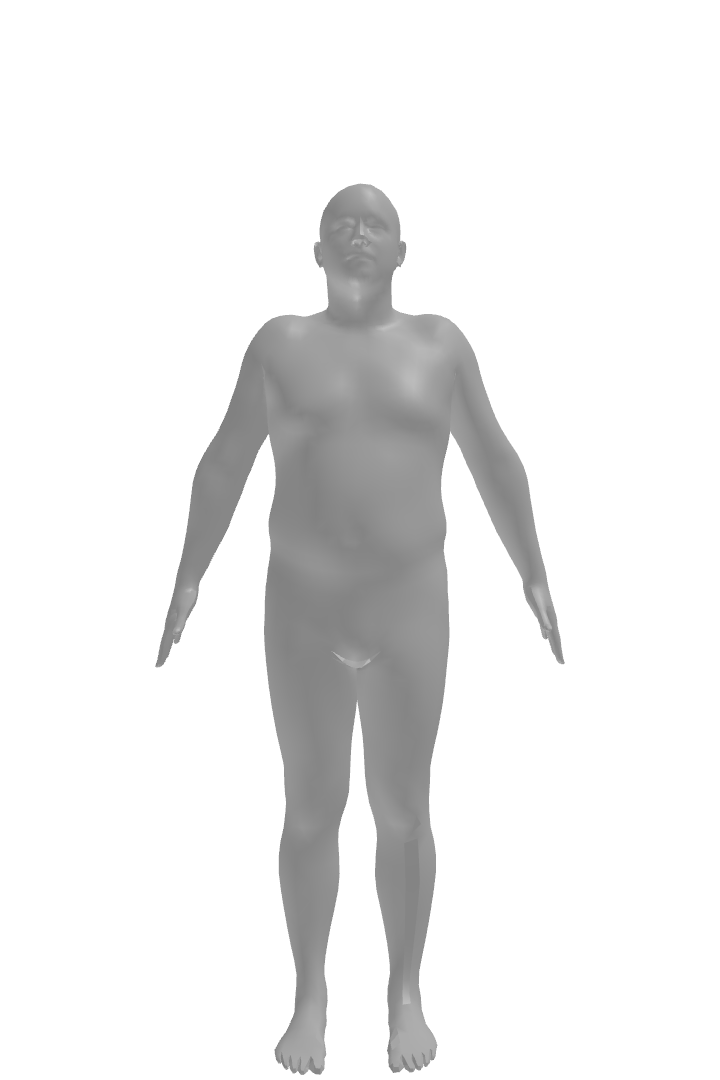
\includegraphics[width=120pt]{files/patient_2/2_11}
    \linebreak
    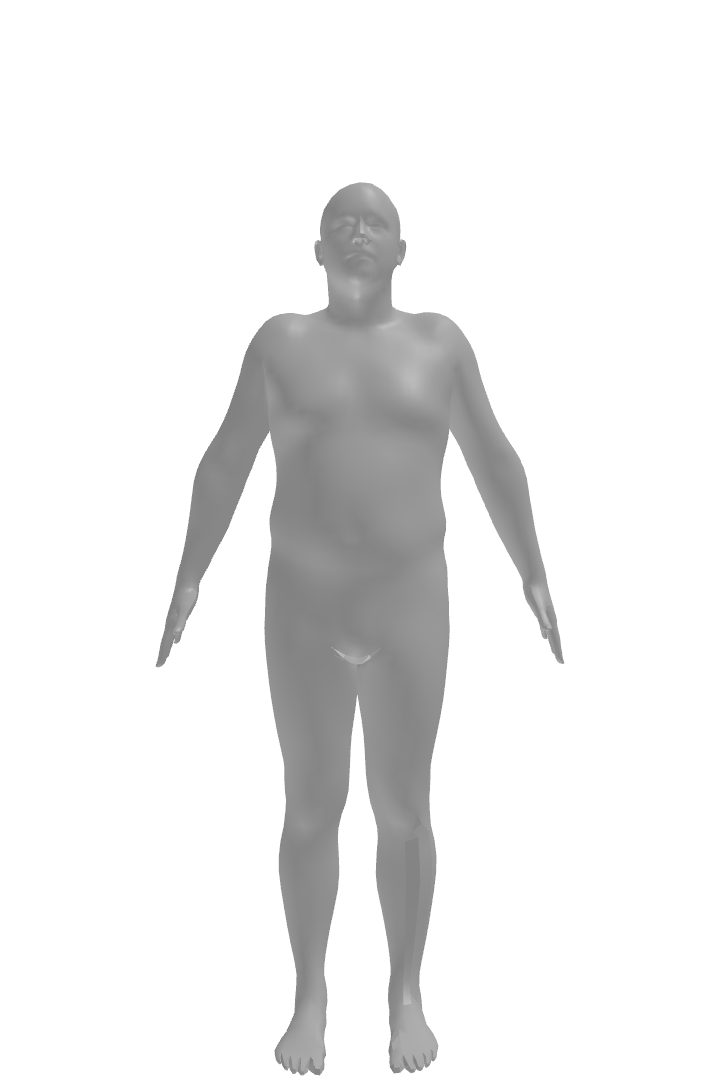
\includegraphics[width=120pt]{files/patient_2/2_predicted}
    \caption[Reconstructed 3D model of the patient's body]{Reconstructed 3D model of the patient's body. The last image is the model's prediction after one month from the last session. There are a total of 74 days between the first and last session.}
    \label{fig:patient-body-model}
\end{figure}

The results obtained provide an initial understanding of the model's
performance and will be further examined and discussed in the subsequent
chapter.
%%%%%%%%%%%%%%%%%%%%%%%%%%%%%%%%%%%%%%%%%%%%%%%%%%%%%%%%%%%%%%%%%%%%%%%%
% Plantilla TFG/TFM
% Escuela Politécnica Superior de la Universidad de Alicante
% Realizado por: Jose Manuel Requena Plens
% Contacto: info@jmrplens.com / Telegram:@jmrplens
%%%%%%%%%%%%%%%%%%%%%%%%%%%%%%%%%%%%%%%%%%%%%%%%%%%%%%%%%%%%%%%%%%%%%%%%

\chapter{Results}\label{chap:results}

In this chapter we will go through the results obtained from the experiments
performed in the previous chapter. We will start by evaluating the predictive
performance of our model, followed by a discussion of the results and their
implications.

\section{Evaluation}

\begin{figure}
    \centering
    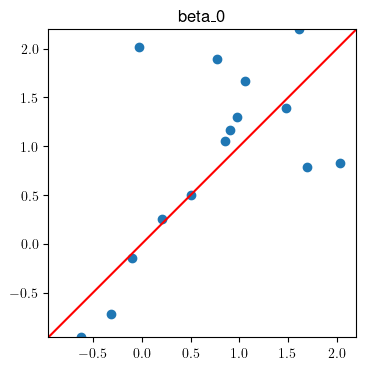
\includegraphics[width=0.3\textwidth]{files/plots/scatter/beta_0.png}
    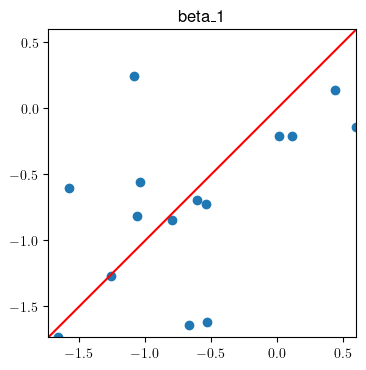
\includegraphics[width=0.3\textwidth]{files/plots/scatter/beta_1.png}
    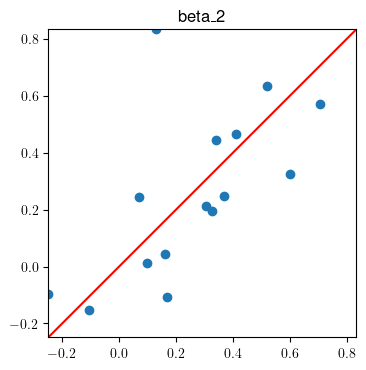
\includegraphics[width=0.3\textwidth]{files/plots/scatter/beta_2.png}
    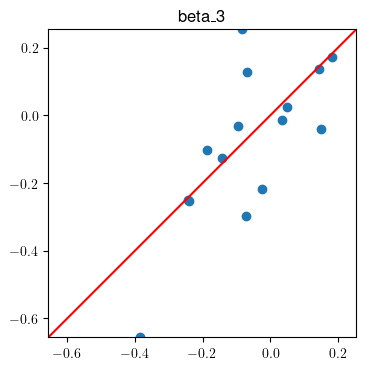
\includegraphics[width=0.3\textwidth]{files/plots/scatter/beta_3.png}
    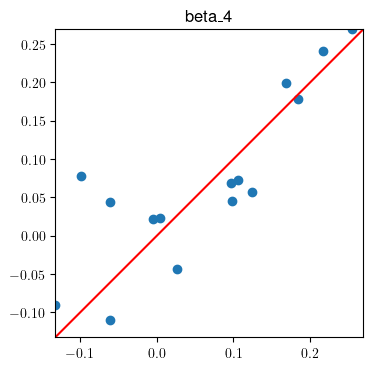
\includegraphics[width=0.3\textwidth]{files/plots/scatter/beta_4.png}
    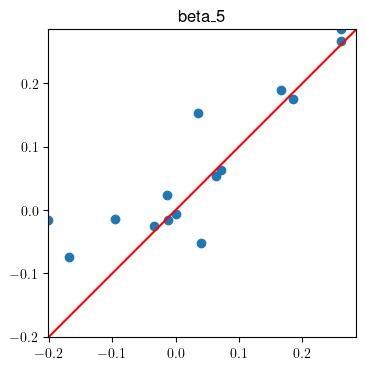
\includegraphics[width=0.3\textwidth]{files/plots/scatter/beta_5.png}
    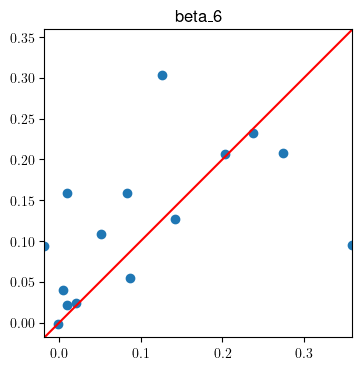
\includegraphics[width=0.3\textwidth]{files/plots/scatter/beta_6.png}
    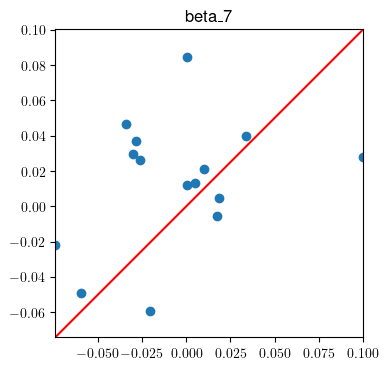
\includegraphics[width=0.3\textwidth]{files/plots/scatter/beta_7.png}
    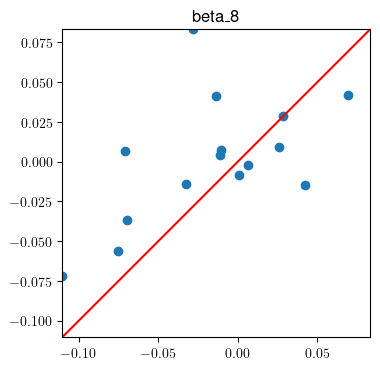
\includegraphics[width=0.3\textwidth]{files/plots/scatter/beta_8.png}
    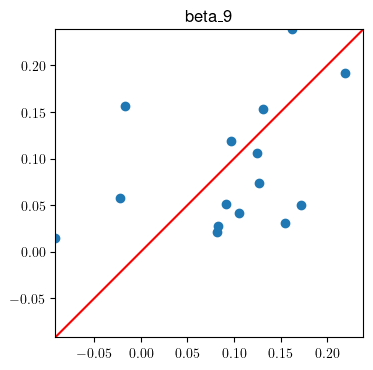
\includegraphics[width=0.3\textwidth]{files/plots/scatter/beta_9.png}
    \caption{Predictions vs ground truth}
    \label{fig:scatter}
\end{figure}

\subsection{Quantitative results}

The mean \gls{mae} of the model in the test set when predicting the $\beta$
parameter is \textbf{0.064}. Figure \ref{fig:scatter} shows the predictions of
the model vs the ground truth, and Table \ref{tab:mae} shows the \gls{mae} for
each $\beta$. We can see that the model is able to predict the correct value in
most cases, but it has some problems with outliers.

\begin{table}[h]
    \centering
    \caption{\gls{mae} for each $\beta$ parameter}
    \begin{tabular}{ c c }
        \toprule
        \textbf{Feature} & \textbf{MAE} \\
        \midrule
        $\beta_1$        & 0.107        \\
        $\beta_2$        & 0.129        \\
        $\beta_3$        & 0.076        \\
        $\beta_4$        & 0.065        \\
        $\beta_5$        & 0.017        \\
        $\beta_6$        & 0.027        \\
        $\beta_7$        & 0.025        \\
        $\beta_8$        & 0.021        \\
        $\beta_9$        & 0.041        \\
        $\beta_{10}$     & 0.025        \\
        \bottomrule
        \label{tab:mae}
    \end{tabular}
\end{table}

\subsection{Qualitative results}
\begin{figure}[h]
    \centering
    \begin{subfigure}{\textwidth}
        \centering
        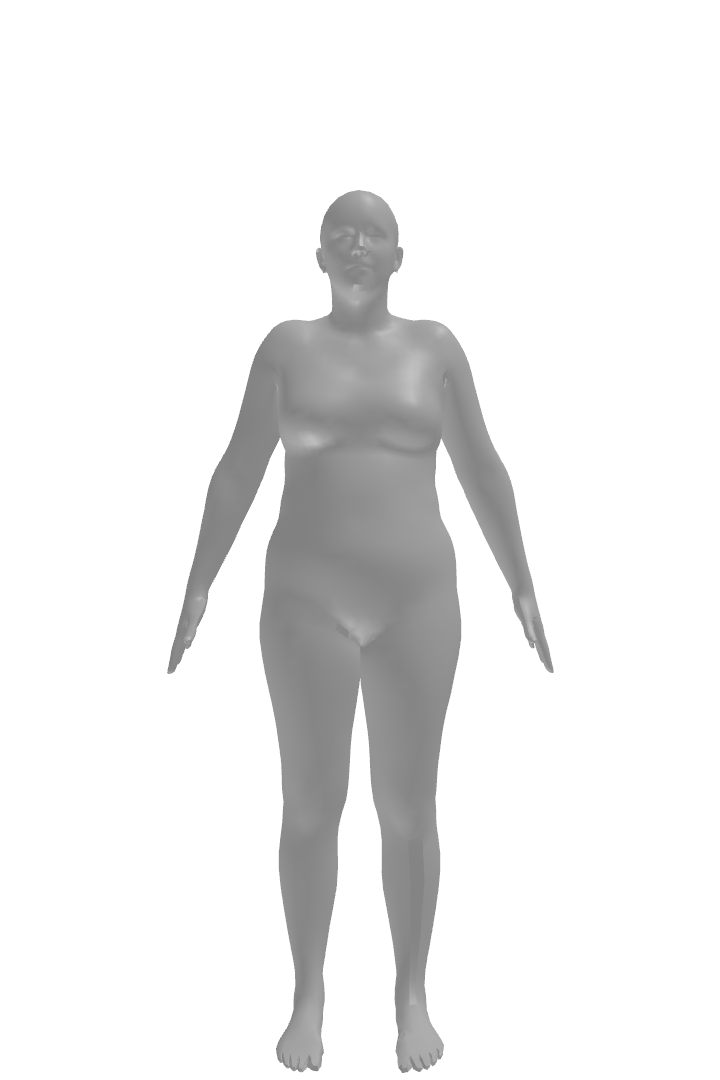
\includegraphics[width=60pt]{files/patients/9_2}
        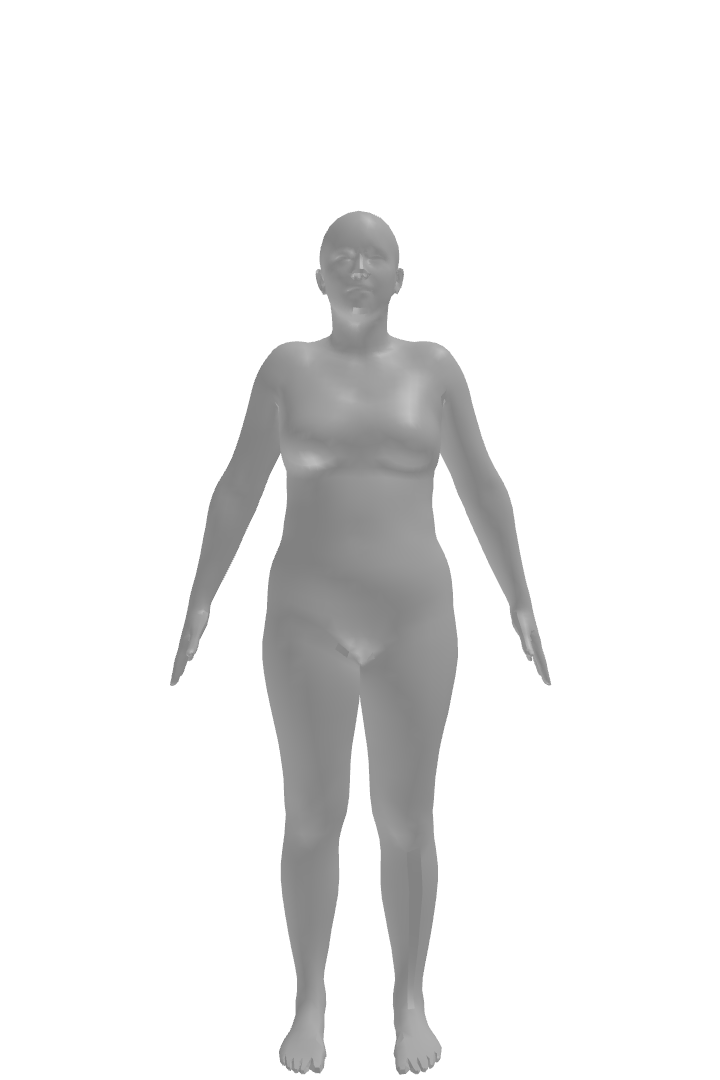
\includegraphics[width=60pt]{files/patients/9_3}
        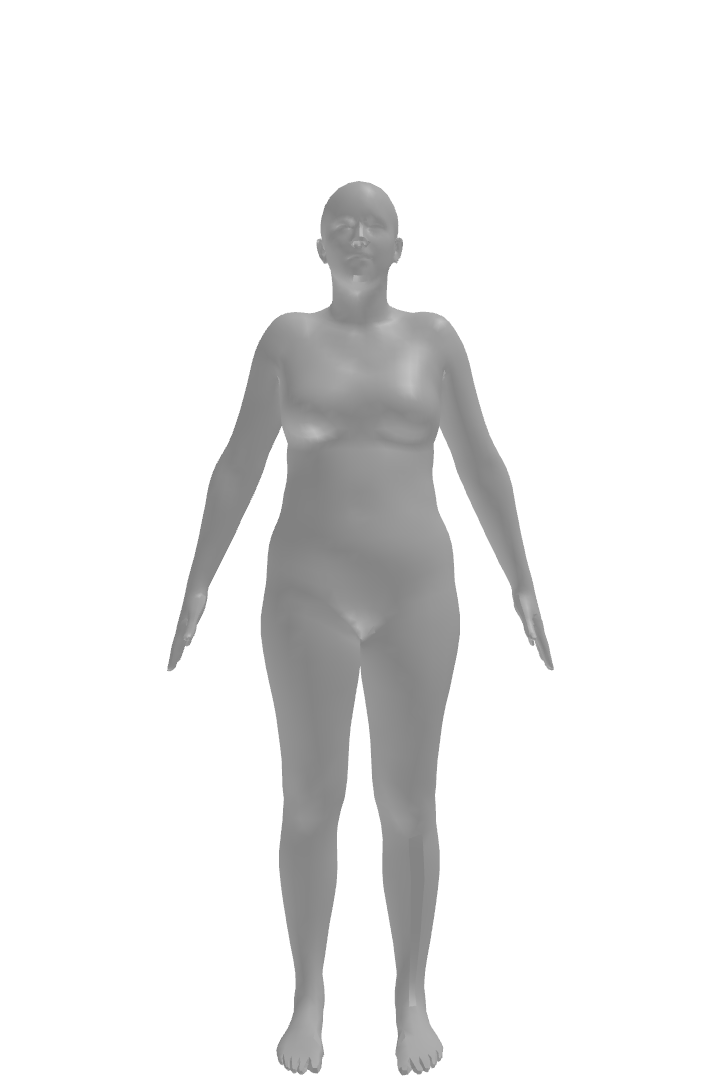
\includegraphics[width=60pt]{files/patients/9_4}
        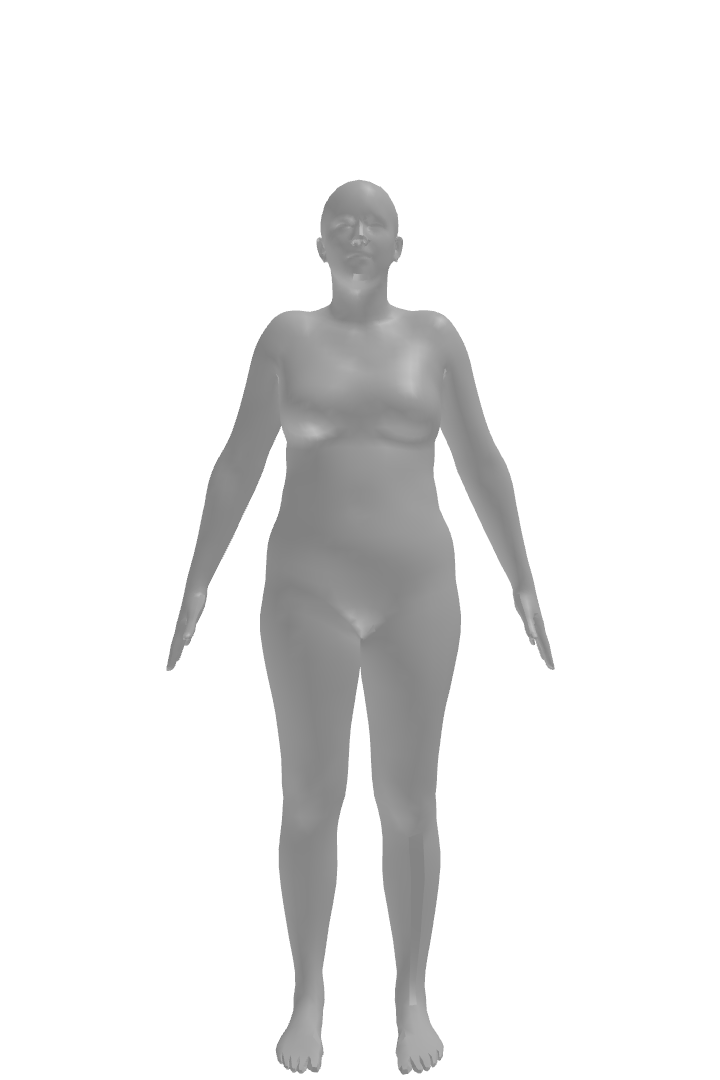
\includegraphics[width=60pt]{files/patients/9_5}
        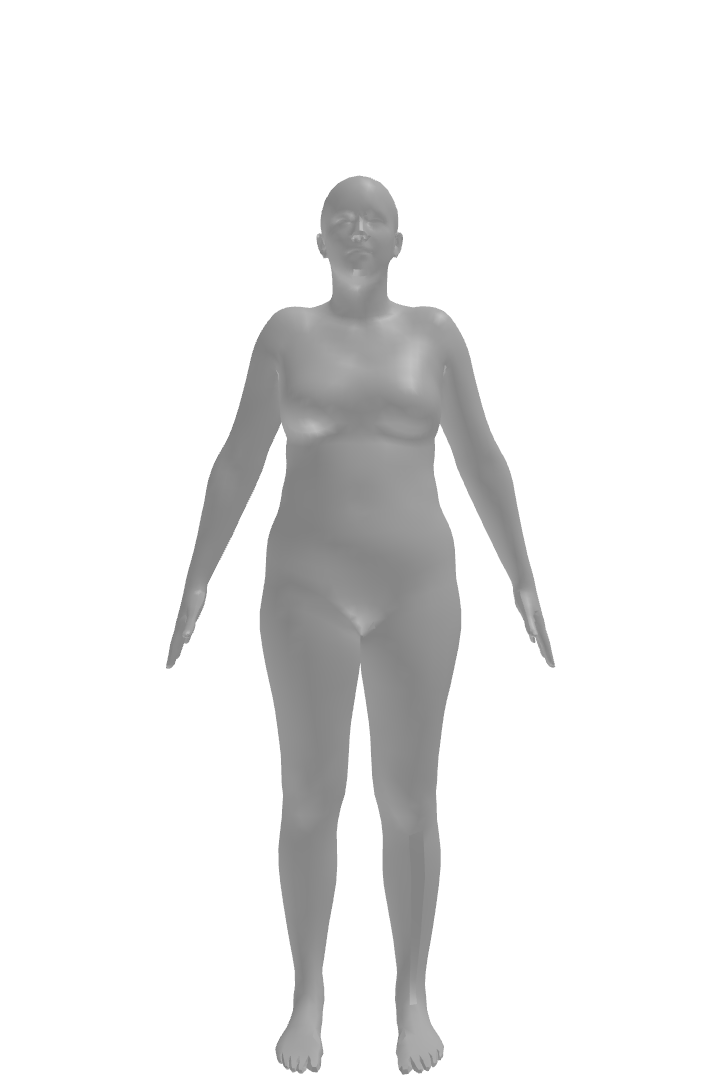
\includegraphics[width=60pt]{files/patients/9_6}
        \hspace{10pt}
        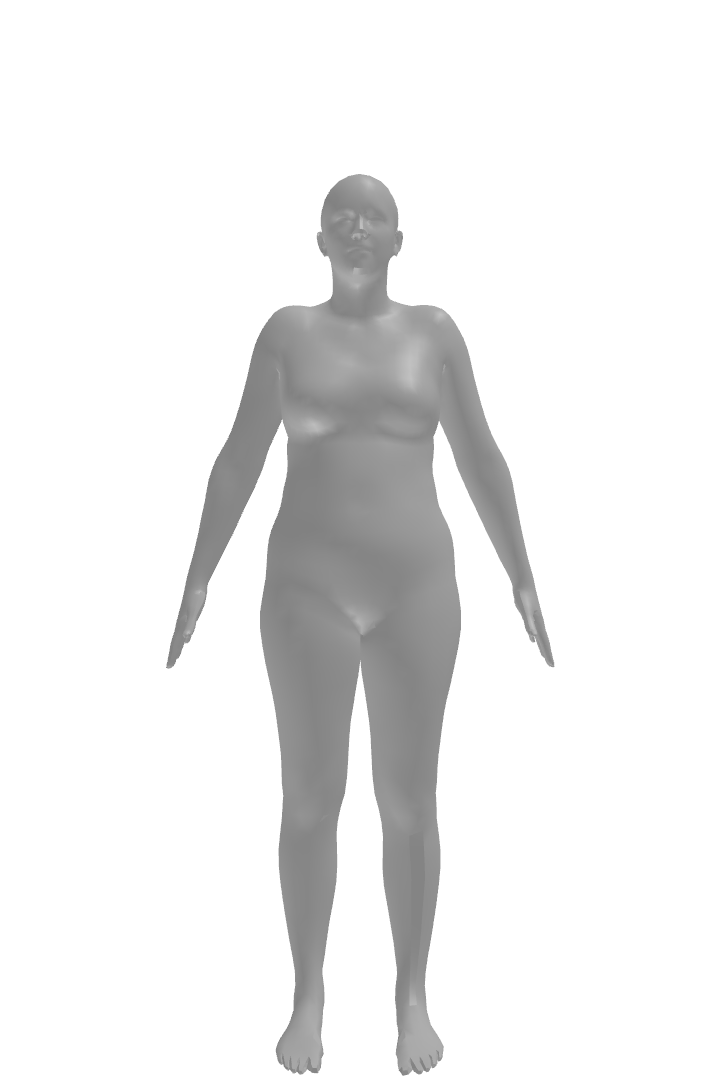
\includegraphics[width=60pt]{files/patients/9_predicted}
    \end{subfigure}
    \linebreak
    \begin{subfigure}{\textwidth}
        \centering
        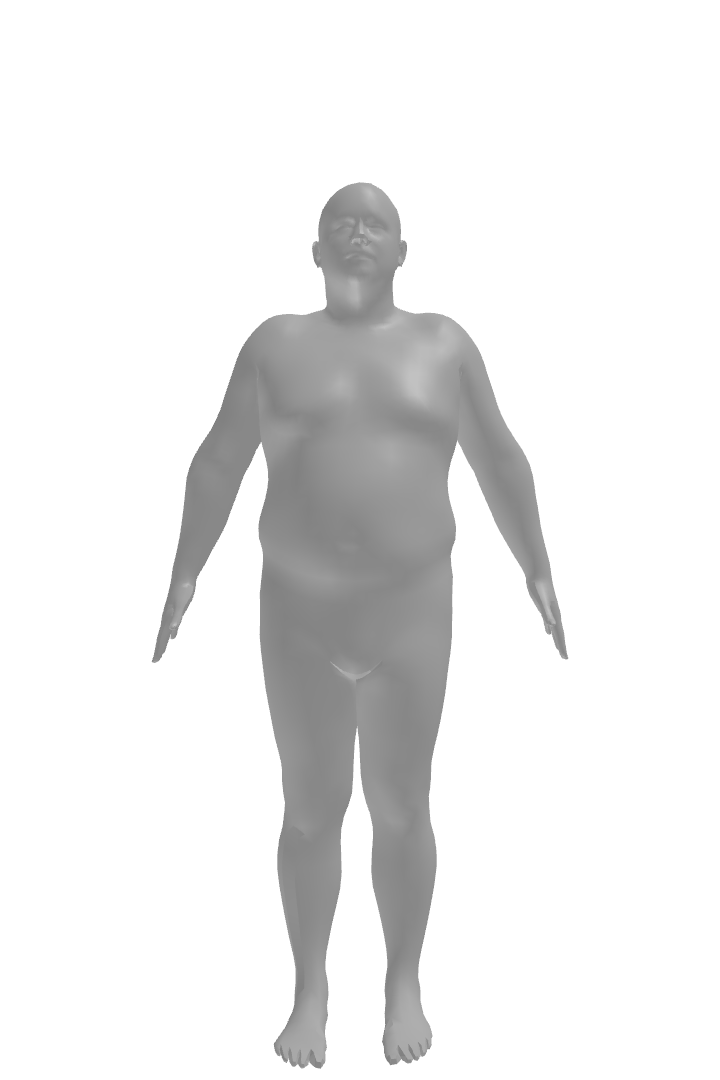
\includegraphics[width=60pt]{files/patients/128_1}
        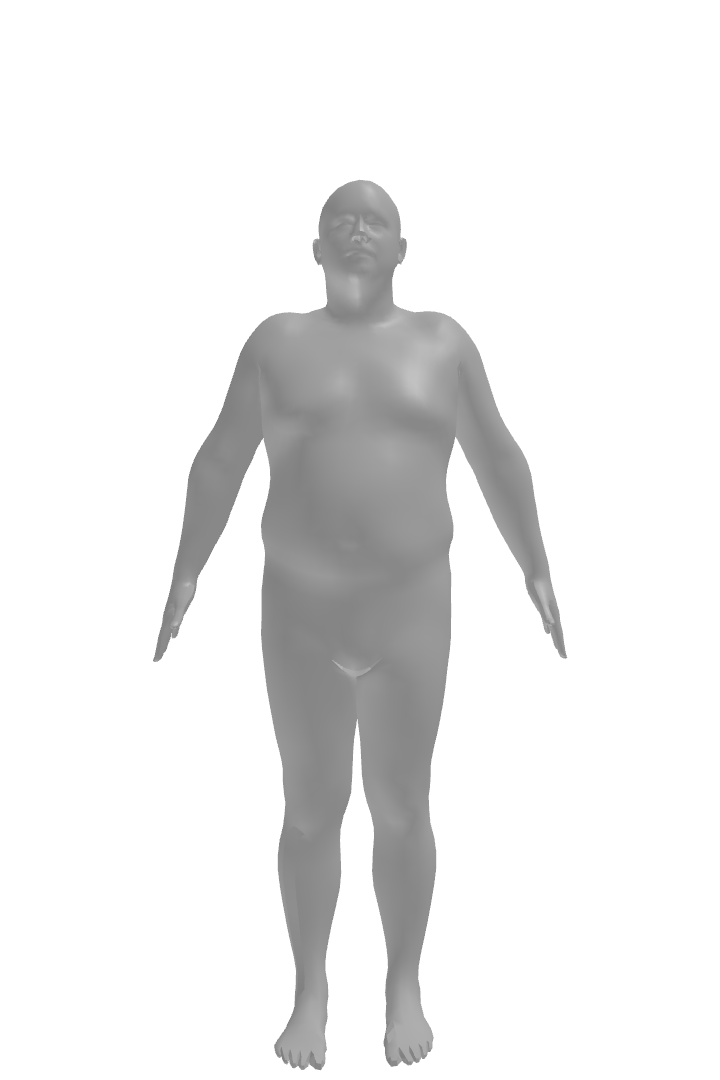
\includegraphics[width=60pt]{files/patients/128_2}
        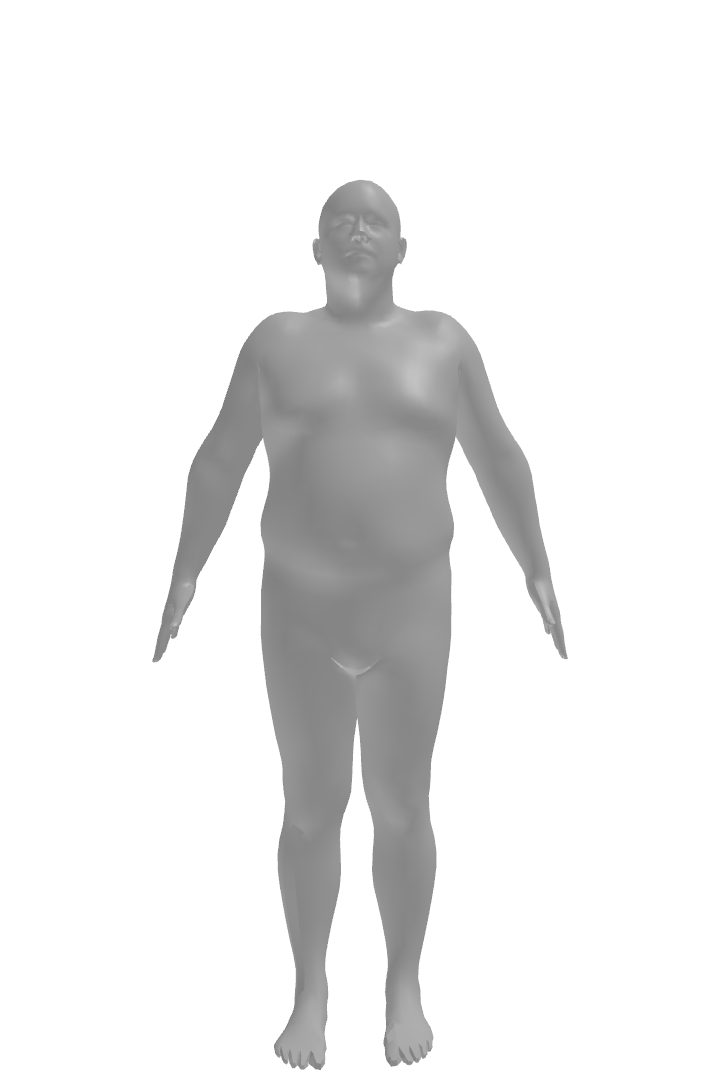
\includegraphics[width=60pt]{files/patients/128_3}
        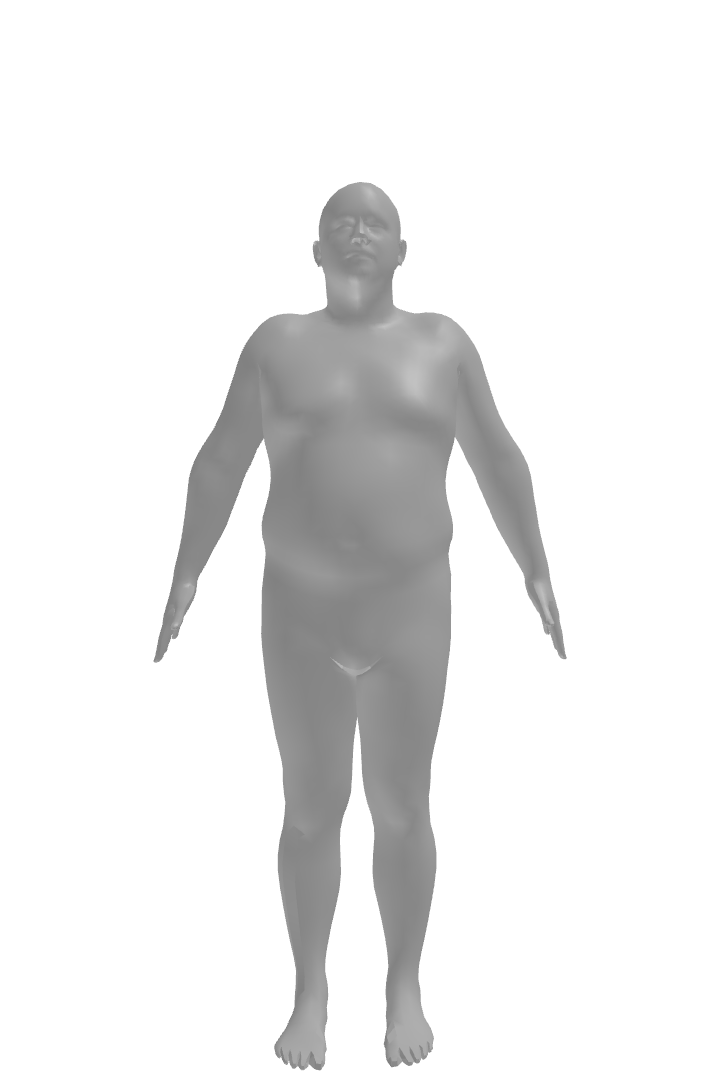
\includegraphics[width=60pt]{files/patients/128_4}
        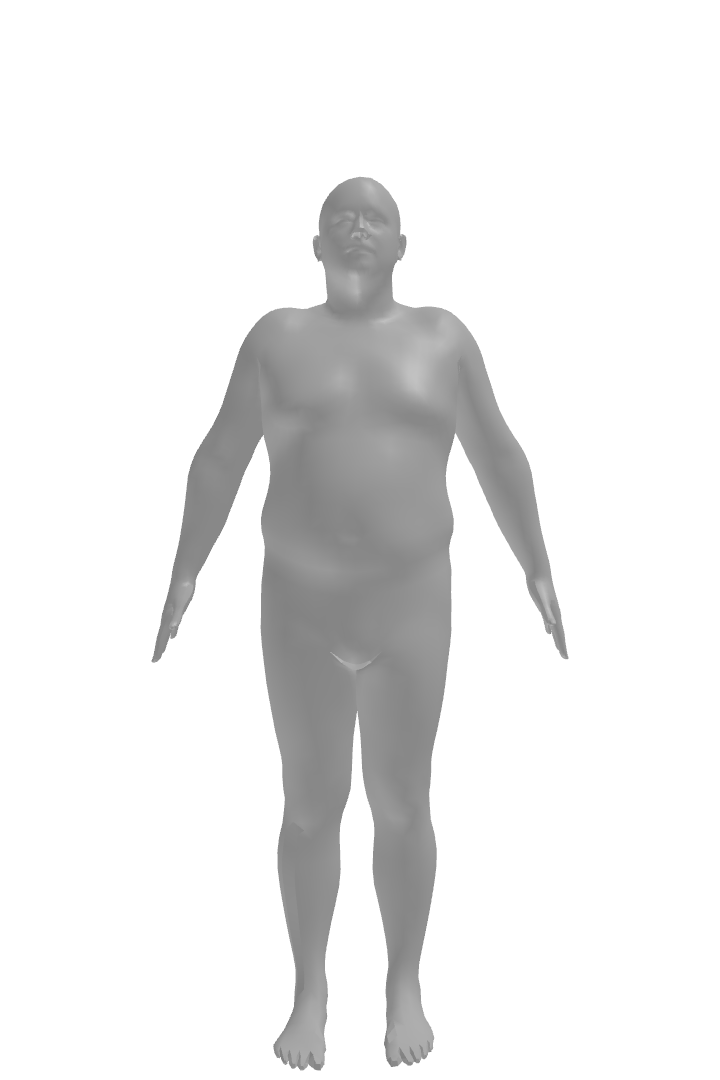
\includegraphics[width=60pt]{files/patients/128_5}
        \hspace{10pt}
        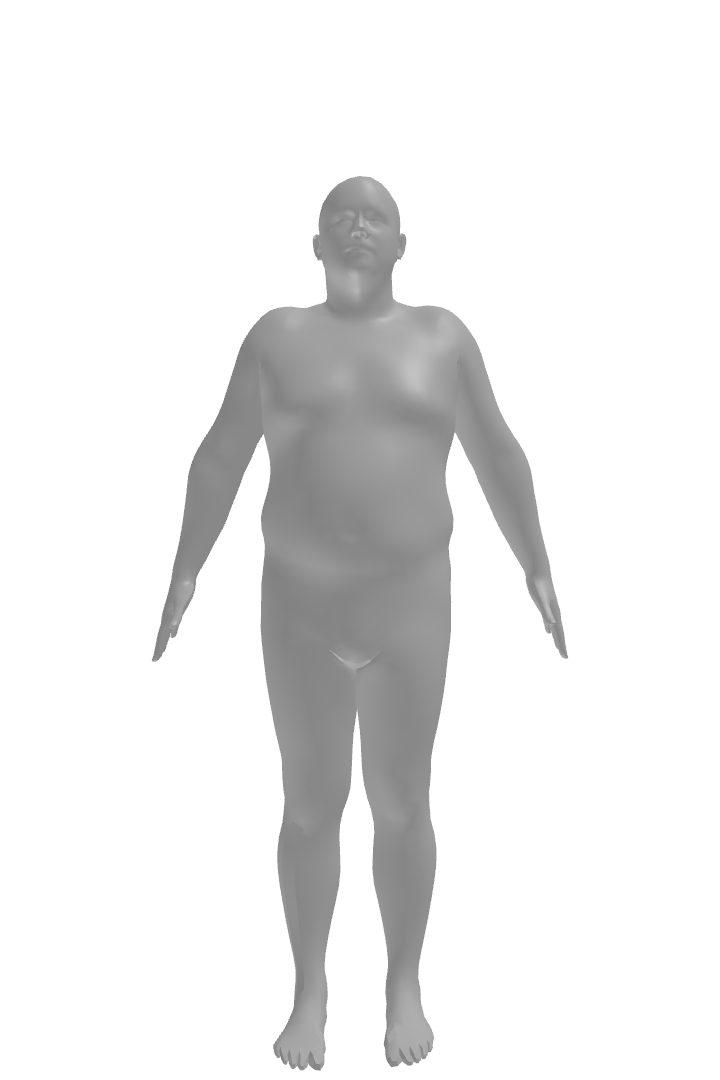
\includegraphics[width=60pt]{files/patients/128_predicted}
    \end{subfigure}
    \caption{Predicted bodies for two patients.}
\end{figure}

\section{Discussion}

\begin{figure}[h]
    \centering
    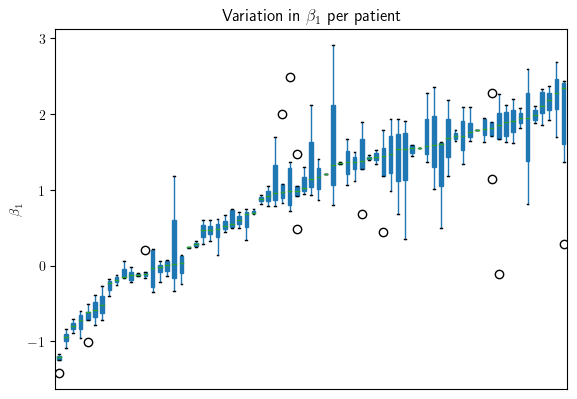
\includegraphics{files/beta_1_var.png}
    \caption{Variation of $\beta_1$ in the dataset per patient.}
    \label{fig:beta-var}
\end{figure}

One of the main problems of the model is that it has a lot of variance in
$\beta_1$. This parameter controls the overall height of the person (Figure
\ref{fig:beta-1-vis}). This has the effect of making the generated human bodies
vary in height, which is not desirable.

This is probably due to the fact that the training data has a lot of variance
in height, which is probably due to scanning error or our method of extracting
the \gls{smpl} parameters from the scans. Figure \ref{fig:beta-var} shows the
variation of $\beta_1$ in the dataset per patient.

To mitigate this problem, several solutions can be explored. One potential
solution is the improvement of data preprocessing, specifically in the
extraction of the SMPL parameters from the scans. By refining this process, the
quality of the training data can be significantly enhanced, reducing the
variance in the $\beta_1$ parameter and leading to more accurate predictions.

Alternatively, we could consider incorporating a form of regularization into
our model specifically targeted at controlling the variation in the height
parameter. By including a penalty term in our loss function that encourages
consistency in the height parameter, we can influence the model to maintain
more stable height predictions across sequences.

Finally, it is also possible to investigate the use of post-processing
techniques. For instance, once the model makes a prediction, we can adjust the
$\beta_1$ value based on a running average from previous sessions, thus
ensuring more consistency in the predicted height.
%%%%%%%%%%%%%%%%%%%%%%%%%%%%%%%%%%%%%%%%%%%%%%%%%%%%%%%%%%%%%%%%%%%%%%%%
% Plantilla TFG/TFM
% Escuela Politécnica Superior de la Universidad de Alicante
% Realizado por: Jose Manuel Requena Plens
% Contacto: info@jmrplens.com / Telegram:@jmrplens
%%%%%%%%%%%%%%%%%%%%%%%%%%%%%%%%%%%%%%%%%%%%%%%%%%%%%%%%%%%%%%%%%%%%%%%%

\chapter{Conclusion}\label{conclusion}

This work has paved the way for an innovative approach to predicting changes in
body shape during weight loss treatment, using machine learning models and the
data gathered from the previous study. Our prediction model based on \gls{smpl}
and a \gls{lstm}-based neural network successfully demonstrated its ability to
approximate the expected changes in body shape before the conclusion of the
weight loss treatment, which could potentially lead to improved adherence to
treatment plans.

However, our study was not without limitations. The model's performance was
constrained by the quantity and quality of data available. Our dataset
consisted of approximately 200 sessions from 80 patients, which, while
substantial, might not fully capture the wide range of variability in human
body shapes and weight loss patterns. Moreover, outliers and missing data,
which had to be cleaned from our dataset, posed additional challenges.

In future work, several improvements and expansions can be explored:

\begin{itemize}
    \item \textbf{Data collection}: Patients could submit images instead of requiring 3D scans. This approach would allow for increased data collection, while also reducing friction for the patient. We can also consider developing a method to generate 3D models from these images.
    \item \textbf{Neural network architecture}: While we opted for a \gls{lstm}
          architecture due to the nature of our data, other neural network architectures,
          such as Transformers, could be explored for potential improvements in
          prediction performance.
    \item \textbf{Parametric models}: Other parametric models like STAR could
          be considered as alternatives or complements to the \gls{smpl}
          model we used. They might offer different advantages or better fit
          the data depending on the specific conditions and requirements.

    \item \textbf{Rendering output}: An exploration of smplpix for 2D
          rendering output might provide an alternative approach for generating
          visualization of predicted body changes.
\end{itemize}

%%%%
% CONTENIDO. BIBLIOGRAFÍA.
%%%%
\nocite{*} %incluye TODOS los documentos de la base de datos bibliográfica sean o no citados en el texto
\bibliographystyle{apalike}
\bibliography{bibliography/bibliography} % Archivo que contiene la bibliografía
% \bibliographystyle{abbrv}

%%%%
% CONTENIDO. LISTA DE ACRÓNIMOS. Comenta las líneas si no lo deseas incluir.
%%%%
% Incluye el listado de acrónimos utilizados en el trabajo. 
\printglossary[style=modsuper,type=\acronymtype,title={List of Acronyms}]
% Añade el resto de acrónimos si así se desea. Si no elimina el comando siguiente
% \glsaddallunused

%%%%
% CONTENIDO. Anexos - Añade o elimina según tus necesidades
%%%%
\appendix % Inicio de los apéndices
%%%%%%%%%%%%%%%%%%%%%%%%%%%%%%%%%%%%%%%%%%%%%%%%%%%%%%%%%%%%%%%%%%%%%%%%
% Plantilla TFG/TFM
% Escuela Politécnica Superior de la Universidad de Alicante
% Realizado por: Jose Manuel Requena Plens
% Contacto: info@jmrplens.com / Telegram:@jmrplens
%%%%%%%%%%%%%%%%%%%%%%%%%%%%%%%%%%%%%%%%%%%%%%%%%%%%%%%%%%%%%%%%%%%%%%%%

\chapter{Annex I}
% Aquí vendría el anexo I 

\def\betaVar{3}
\def\imgWidth{0.3\textwidth}
\def\betaWidth{\textwidth}

\begin{figure}[ht!]
    \centering
    \begin{minipage}[b]{\textwidth}
        \centering
        \includegraphics[width=\imgWidth]{files/visualize_betas/beta_0_-\betaVar_m}
        \includegraphics[width=\imgWidth]{files/visualize_betas/baseline_m}
        \includegraphics[width=\imgWidth]{files/visualize_betas/beta_0_\betaVar_m}
        \linebreak
        \includegraphics[width=\imgWidth]{files/visualize_betas/beta_0_-\betaVar_f}
        \includegraphics[width=\imgWidth]{files/visualize_betas/baseline_f}
        \includegraphics[width=\imgWidth]{files/visualize_betas/beta_0_\betaVar_f}
        \caption[Effect of varying $\beta_1$ in SMPL.]{$\beta_1 = [-\betaVar, 0, +\betaVar]$.}
        \label{fig:beta-1-vis}
    \end{minipage}
\end{figure}

\begin{figure}[ht!]
    \centering

    \begin{minipage}[b]{\textwidth}
        \centering
        \includegraphics[width=\imgWidth]{files/visualize_betas/beta_1_-\betaVar_m}
        \includegraphics[width=\imgWidth]{files/visualize_betas/baseline_m}
        \includegraphics[width=\imgWidth]{files/visualize_betas/beta_1_\betaVar_m}
        \linebreak
        \includegraphics[width=\imgWidth]{files/visualize_betas/beta_1_-\betaVar_f}
        \includegraphics[width=\imgWidth]{files/visualize_betas/baseline_f}
        \includegraphics[width=\imgWidth]{files/visualize_betas/beta_1_\betaVar_f}
        \caption[Effect of varying $\beta_2$ in SMPL.]{$\beta_2 = [-\betaVar, 0, +\betaVar]$.}
    \end{minipage}
\end{figure}

\begin{figure}[ht!]
    \centering

    \begin{minipage}[b]{\textwidth}
        \centering
        \includegraphics[width=\imgWidth]{files/visualize_betas/beta_2_-\betaVar_m}
        \includegraphics[width=\imgWidth]{files/visualize_betas/baseline_m}
        \includegraphics[width=\imgWidth]{files/visualize_betas/beta_2_\betaVar_m}
        \linebreak
        \includegraphics[width=\imgWidth]{files/visualize_betas/beta_2_-\betaVar_f}
        \includegraphics[width=\imgWidth]{files/visualize_betas/baseline_f}
        \includegraphics[width=\imgWidth]{files/visualize_betas/beta_2_\betaVar_f}
        \caption[Effect of varying $\beta_3$ in SMPL.]{$\beta_3 = [-\betaVar, 0, +\betaVar]$.}
    \end{minipage}
\end{figure}

\begin{figure}[ht!]
    \centering

    \begin{minipage}[b]{\textwidth}
        \centering
        \includegraphics[width=\imgWidth]{files/visualize_betas/beta_3_-\betaVar_m}
        \includegraphics[width=\imgWidth]{files/visualize_betas/baseline_m}
        \includegraphics[width=\imgWidth]{files/visualize_betas/beta_3_\betaVar_m}
        \linebreak
        \includegraphics[width=\imgWidth]{files/visualize_betas/beta_3_-\betaVar_f}
        \includegraphics[width=\imgWidth]{files/visualize_betas/baseline_f}
        \includegraphics[width=\imgWidth]{files/visualize_betas/beta_3_\betaVar_f}
        \caption[Effect of varying $\beta_4$ in SMPL.]{$\beta_4 = [-\betaVar, 0, +\betaVar]$.}
    \end{minipage}
\end{figure}

\begin{figure}[ht!]
    \centering

    \begin{minipage}[b]{\textwidth}
        \centering
        \includegraphics[width=\imgWidth]{files/visualize_betas/beta_4_-\betaVar_m}
        \includegraphics[width=\imgWidth]{files/visualize_betas/baseline_m}
        \includegraphics[width=\imgWidth]{files/visualize_betas/beta_4_\betaVar_m}
        \linebreak
        \includegraphics[width=\imgWidth]{files/visualize_betas/beta_4_-\betaVar_f}
        \includegraphics[width=\imgWidth]{files/visualize_betas/baseline_f}
        \includegraphics[width=\imgWidth]{files/visualize_betas/beta_4_\betaVar_f}
        \caption[Effect of varying $\beta_5$ in SMPL.]{$\beta_5 = [-\betaVar, 0, +\betaVar]$.}
    \end{minipage}
\end{figure}

\begin{figure}[ht!]
    \centering

    \begin{minipage}[b]{\textwidth}
        \centering
        \includegraphics[width=\imgWidth]{files/visualize_betas/beta_5_-\betaVar_m}
        \includegraphics[width=\imgWidth]{files/visualize_betas/baseline_m}
        \includegraphics[width=\imgWidth]{files/visualize_betas/beta_5_\betaVar_m}
        \linebreak
        \includegraphics[width=\imgWidth]{files/visualize_betas/beta_5_-\betaVar_f}
        \includegraphics[width=\imgWidth]{files/visualize_betas/baseline_f}
        \includegraphics[width=\imgWidth]{files/visualize_betas/beta_5_\betaVar_f}
        \caption[Effect of varying $\beta_6$ in SMPL.]{$\beta_6 = [-\betaVar, 0, +\betaVar]$.}
    \end{minipage}
\end{figure}

\begin{figure}[ht!]
    \centering

    \begin{minipage}[b]{\textwidth}
        \centering
        \includegraphics[width=\imgWidth]{files/visualize_betas/beta_6_-\betaVar_m}
        \includegraphics[width=\imgWidth]{files/visualize_betas/baseline_m}
        \includegraphics[width=\imgWidth]{files/visualize_betas/beta_6_\betaVar_m}
        \linebreak
        \includegraphics[width=\imgWidth]{files/visualize_betas/beta_6_-\betaVar_f}
        \includegraphics[width=\imgWidth]{files/visualize_betas/baseline_f}
        \includegraphics[width=\imgWidth]{files/visualize_betas/beta_6_\betaVar_f}
        \caption[Effect of varying $\beta_7$ in SMPL.]{$\beta_7 = [-\betaVar, 0, +\betaVar]$.}
    \end{minipage}
\end{figure}

\begin{figure}[ht!]
    \centering

    \begin{minipage}[b]{\textwidth}
        \centering
        \includegraphics[width=\imgWidth]{files/visualize_betas/beta_7_-\betaVar_m}
        \includegraphics[width=\imgWidth]{files/visualize_betas/baseline_m}
        \includegraphics[width=\imgWidth]{files/visualize_betas/beta_7_\betaVar_m}
        \linebreak
        \includegraphics[width=\imgWidth]{files/visualize_betas/beta_7_-\betaVar_f}
        \includegraphics[width=\imgWidth]{files/visualize_betas/baseline_f}
        \includegraphics[width=\imgWidth]{files/visualize_betas/beta_7_\betaVar_f}
        \caption[Effect of varying $\beta_8$ in SMPL.]{$\beta_8 = [-\betaVar, 0, +\betaVar]$.}
    \end{minipage}
\end{figure}

\begin{figure}[ht!]
    \centering

    \begin{minipage}[b]{\textwidth}
        \centering
        \includegraphics[width=\imgWidth]{files/visualize_betas/beta_8_-\betaVar_m}
        \includegraphics[width=\imgWidth]{files/visualize_betas/baseline_m}
        \includegraphics[width=\imgWidth]{files/visualize_betas/beta_8_\betaVar_m}
        \linebreak
        \includegraphics[width=\imgWidth]{files/visualize_betas/beta_8_-\betaVar_f}
        \includegraphics[width=\imgWidth]{files/visualize_betas/baseline_f}
        \includegraphics[width=\imgWidth]{files/visualize_betas/beta_8_\betaVar_f}
        \caption[Effect of varying $\beta_9$ in SMPL.]{$\beta_9 = [-\betaVar, 0, +\betaVar]$.}
    \end{minipage}
\end{figure}

\begin{figure}[ht!]
    \centering

    \begin{minipage}[b]{\textwidth}
        \centering
        \includegraphics[width=\imgWidth]{files/visualize_betas/beta_9_-\betaVar_m}
        \includegraphics[width=\imgWidth]{files/visualize_betas/baseline_m}
        \includegraphics[width=\imgWidth]{files/visualize_betas/beta_9_\betaVar_m}
        \linebreak
        \includegraphics[width=\imgWidth]{files/visualize_betas/beta_9_-\betaVar_f}
        \includegraphics[width=\imgWidth]{files/visualize_betas/baseline_f}
        \includegraphics[width=\imgWidth]{files/visualize_betas/beta_9_\betaVar_f}
        \caption[Effect of varying $\beta_{10}$ in SMPL.]{$\beta_{10} = [-\betaVar, 0, +\betaVar]$.}
        \label{fig:beta-10-vis}
    \end{minipage}
\end{figure}


%%%%%%%%%%%%%%%%%%%%%%%%%%%%%%%%%%%%%%%%%%%%%%%%%%%%%%%%%%%%%%%%%%%%%%%%
% Plantilla TFG/TFM
% Escuela Politécnica Superior de la Universidad de Alicante
% Realizado por: Jose Manuel Requena Plens
% Contacto: info@jmrplens.com / Telegram:@jmrplens
%%%%%%%%%%%%%%%%%%%%%%%%%%%%%%%%%%%%%%%%%%%%%%%%%%%%%%%%%%%%%%%%%%%%%%%%

% Ejemplo de páginas en horizontal y vertical

% \chapter{Páginas horizontales}
% Aquí se muestra cómo incluir páginas en horizontal.

% Esta página está en vertical\\
% \clearpage % Nueva página

% \begin{landscape} % Inicia modo horizontal

% Esta página está en horizontal\\
% \clearpage % Nueva página

% Esta página también está en horizontal\\

% \end{landscape} % Finaliza modo horizontal
% \clearpage % Nueva página

% Esta página está de nuevo en vertical\\


%%%%%%%%%%%%%%%%%%%%%%%%%%%%%%%%%%%%%%%%%%%%%%%%%%%%%%%%%%%%%%%%%%%%%%%%
% Plantilla TFG/TFM
% Escuela Politécnica Superior de la Universidad de Alicante
% Realizado por: Jose Manuel Requena Plens
% Contacto: info@jmrplens.com / Telegram:@jmrplens
%%%%%%%%%%%%%%%%%%%%%%%%%%%%%%%%%%%%%%%%%%%%%%%%%%%%%%%%%%%%%%%%%%%%%%%%

% Ejemplo de inclusión de páginas de un PDF

\chapter{Importar PDF}

A continuación se muestra una página importada de un PDF externo. Observar los comentarios en el código de este anexo para más información. También puedes leer el manual con todas las opciones en \url{http://osl.ugr.es/CTAN/macros/latex/contrib/pdfpages/pdfpages.pdf}.

\includepdf[pages={1}]{archivos/ES_a_DF7_Agg_Alicante.pdf}

% Para incluir una página:
% [pages={0}] % Donde '0' es el número de la pagina del PDF que se quiere incluir

% Para incluir varias páginas consecutivas
% [pages={1-4}] % Con estos valores importa de la página 1 a la 4.

% Para incluir varias páginas salteadas
% [pages={1,4,7,10}] % Incluye las páginas 1,4,7 y 10

% Para incluir todo el documento PDF
% [pages=-]

% Si ademas de pages=... se incluye landscape, se importa en horizontal
% [pages{1},landscape]

\end{document}